%%%*******************************************************************************
%  Classe Latex THEOPRAX, Version 0.0.0 31/10/2017
%
%  Define as normas e estilo das dissertações, teses ou tcc do SENAI CIMATEC
%
%%%-------------------------------------------------------------------------------

%%%-------------------------------------------------------------------------------
% Changes log
%%%-------------------------------------------------------------------------------
% Version 0.0.0 - 00/00/2000
% - https://v2.overleaf.com/project/5b8f04cbb314cb48ffc12abe
%%%-------------------------------------------------------------------------------

%%%-------------------------------------------------------------------------------
%  DOCUMENTATION WITH EXAMPLE
%%%*******************************************************************************

%%%-------------------------------------------------------------------------------
%%% Thesis default options
%%%-------------------------------------------------------------------------------
%\documentclass[subook]{Classes/THEOPRAX}
%\documentclass[sureport]{Classes/THEOPRAX}

%%%-------------------------------------------------------------------------------
%%% Thesis custom options
%%%-------------------------------------------------------------------------------

%%% Fancy page headings
%\documentclass[fancyheadings, subook]{Classes/THEOPRAX}
%\documentclass[fancyheadings, sureport]{Classes/THEOPRAX}

%%% Fancy chapters and sections headings
%\documentclass[fancychapter, subook]{Classes/THEOPRAX}
%\documentclass[fancychapter, sureport]{Classes/THEOPRAX}

%%% Fancy page , chapters and sections headings
%\documentclass[fancyheadings, fancychapter, subook]{Classes/THEOPRAX}
%\documentclass[fancyheadings, fancychapter, sureport]{Classes/THEOPRAX}
\documentclass[fancyheadings, fancychapter, sureport]{Classes/THEOPRAX}

%%%-------------------------------------------------------------------------------
%%% Thesis Commands (ONLY with fancy page headings)
%%%-------------------------------------------------------------------------------

%%%Page header line width
%\footlinewidth{value}

%%%Page footer line width
%\headlinewidth{value}

%%%Page header and footer line width
%\headingslinewidth{value}

%%%Page header and footer lines without text
%\headingslinesonly

%%%The default line width is 0.3pt.
%%%Set the value to 0pt to remove the page header and/or footer line

%%%-------------------------------------------------------------------------------
%%% SUThesis Supported Graphic Formats
%%%-------------------------------------------------------------------------------
% The figures formats supported depend upon the selected output file
% Include your figure without the extention, the SUThesis will automatically
% search the predefined `Figures' directory tree for the right file format.
%
% - The pdfLaTEX (PDF) supports graphics inclusions in PDF, JPG, PNG, and
%   MetaPost (with .mps extention) formats.
%
% - The Latex (DVI) supports graphics inclusions in EPS and PS formats.
%%%-------------------------------------------------------------------------------


%%%-------------------------------------------------------------------------------
%%% Árvore de diretório THEOPRAX
%%%-------------------------------------------------------------------------------
%  Diretório
%       \Classes        (requerido)
%       \Figures        (requerido) --------------------------------->
%       \Figures\PDF    (optional)
%       \Figures\JPG    (optional) Figures located within these
%       \Figures\PNG    (optional) folders are searched automatically
%       \Figures\MPS    (optional)  by the THEOPRAX class.
%       \Figures\EPS    (optional)
%       \Figures\PS     (optional) <--------------------------------
%       \Tables         (requerido)
%       \Others         (requerido)
%       \Chapters       (requerido)
%       \Appendices     (optional)
%       \References     (requerido)
%%%-------------------------------------------------------------------------------

%%%-------------------------------------------------------------------------------
%%% PDF File Summary
%%%-------------------------------------------------------------------------------
\ifpdf
    \hypersetup{backref,
                colorlinks  = true,
                pdftitle    = Modelo de visualização de informação de redes complexas utilizando sistemas de identificação de gestos e realidade virtual,
                pdfauthor   = {Marco Reis, marco.a.reis@gmail.com},
                pdfsubject  = Mestre em Engenharia,
                pdfcreator  = Subtitulo,
                pdfproducer = PDFLatex,
                pdfkeywords = {Palavra-chave1, Palavra-chave2, Palavra-chave3}
    }
 \fi

%%%-------------------------------------------------------------------------------
%%% Required packages
%%%-------------------------------------------------------------------------------
% - ifthen
% - setspace
% - amsmath
% - amsfonts
% - amssymb
% - amsthm
% - eucal
% - graphics
% - fancyhdr
%%%-------------------------------------------------------------------------------

%%%-------------------------------------------------------------------------------
%%% Optional packages
%%%-------------------------------------------------------------------------------
%\usepackage[latin1]{inputenc}
\usepackage[utf8]{inputenc}
\usepackage[brazil]{babel}
\usepackage{longtable}
\usepackage{dcolumn}
\usepackage{multirow}
\usepackage{lscape}
\usepackage{graphicx}
\usepackage{rotating}
\usepackage{float,subfigure}
\usepackage{cite}
\usepackage[left=3cm,top=3cm,right=2cm,bottom=2cm]{geometry}
%\usepackage[alf,abnt-etal-list=5]{abntcite}
\usepackage[alf]{abntex2cite}
\usepackage{ifpdf}
\usepackage{shadow}
\usepackage{wrapfig}
\usepackage[normalem]{ulem}
\usepackage{makeidx} % cria indice remissivo
\usepackage{yfonts}
\makeindex % cria o indice remissivo
%Tables and Figures Caption
\setlength{\LTcapwidth}{\textwidth}





%\usepackage{algorithm}
%\usepackage{algorithmic}




%\newtheorem{theorem}{Teorema}
%\newtheorem{definition}[theorem]{Defini\c{c}\~ao}


%%%-------------------------------------------------------------------------------
%%% Start thesis root document
%%%-------------------------------------------------------------------------------
\begin{document}
    %%----------------------------------------------------------------------------
    %% Define the title page
    %%----------------------------------------------------------------------------
    \university{Centro Universitário SENAI CIMATEC}
%    \faculty{Pro\-gra\-ma de P\'os-gra\-dua\-\c{c}\~ao em Mo\-de\-la\-gem Com\-pu\-ta\-cio\-nal e Tec\-no\-lo\-gia In\-dus\-trial}
    %\faculty{Centro Universitário Senai Cimatec}
%    \school{School of Mathematics}
% ********************************************** TCC ****************
    \course{Engenharia Elétrica}
    \typework{Projeto Theoprax de Conclusão de Curso}
% ********************************************************************
% ********************************************* Mestrado ******************
%    \course{Mestrado em Modelagem Computacional e Tecnologia Industrial}
%    \typework{Disserta\c{c}\~ao de mestrado}
%    \typework{Exame de Qualificação de Mestrado}
% ********************************************** Doutorado ****************
%    \course{Engenharia Elétrica}
%    \typework{Tese de doutorado}
%    \typework{Exame de Qualificação de doutorado}
% ********************************************************************
 \thesistitle{Percepção e suas funcionalidades para um robô de inspeção de linhas de alta tensão}
    \hidevolume
    \thesisvolume{Volume 1 of 1}
    \thesisauthor{Felipe Cafezeiro Plech}
    \thesisauthorr{Luciana Moreno Borges}
    %\thesisauthorrr{James Clerk Maxwell}
   % \thesisauthorrrr{Nikola Tesla}
    \thesisadvisor{Prof. Marco Reis, M.Eng.}
    \hidecoadvisor
    %\thesiscoadvisor{Marco Reis}
    \thesisdegreetitle{Bacharel em Engenharia}
    %\thesisdegreetitle{Doutor em }
%    \thesismonthyear{M\^es de Ano}
    \thesismonthyear{Novembro de 2018}


    \maketitlepage

    %%----------------------------------------------------------------------------
    %% Inserir Folha de rosto, Nota de estilo, folha de assinaturas, dedicatoria
    %%----------------------------------------------------------------------------
    \begin{folharosto}

\begin{center}
\theauthor \\
\theauthorr \\

\end{center}
\ \\
\ \\
\ \\
\ \\
\ \\
\begin{spacing}{2}
   \begin{center}
   {\LARGE {\bf \thetitle}}
   \end{center}
\end{spacing}
\ \\
\ \\
\ \\
\begin{flushright}

   \begin{list}{}{
      \setlength{\leftmargin}{7.5cm}
      \setlength{\rightmargin}{0cm}
      \setlength{\labelwidth}{0pt}
      \setlength{\labelsep}{\leftmargin}}

      \item \thetypework apresentada ao \thefaculty, Curso de \thecourse
      do \theuniversity, como requisito parcial para a obten\c{c}\~ao do
      t\'itulo de {\bf \thedegreetitle}.

      \begin{list}{}{
      \setlength{\leftmargin}{0cm}
      \setlength{\rightmargin}{0cm}
      \setlength{\labelwidth}{0pt}
      \setlength{\labelsep}{\leftmargin}}

      \item \'Area de conhecimento: Interdisciplinar

      \item Orientador: \theadvisor
      \newline \hspace*{2.1cm}  %{\it \theuniversity}

      \end{list}
   \end{list}

\end{flushright}
\ \\
\ \\
\ \\
\ \\
%\begin{spacing}{1.5}
   \begin{center}
   Salvador \par
   \theuniversity \par
   2018
   \end{center}
%\end{spacing}

\end{folharosto}

    %\begin{notaestilo}
Esta \thetypeworkthree foi elaborada considerando as normas de
estilo (i.e. est\'eticas e estruturais) propostas aprovadas pelo
colegiado do \thefacultytwo e est\~ao dispon\'iveis em formato
eletr\^onico ({\it download} na P\'agina Web
http:$//$ead.fieb.org.br$/$portal\_faculdades$/$dissertacoes-e-teses-mcti.html
ou solicita\c{c}\~ao via e-mail \`a secretaria do
programa) e em formato impresso somente para consulta. \\

Ressalta-se que o formato proposto considera diversos itens das
normas da Associa\c{c}\~ao Brasileira de Normas T\'ecnicas (ABNT),
entretanto opta-se, em alguns aspectos, seguir um estilo pr\'oprio
elaborado e amadurecido pelos professores do programa de
p\'os-gradua\c{c}\~ao supracitado.

\end{notaestilo}

    %\begin{folhaassinaturas}

%\thispagestyle{empty}

\def\signature#1#2{\parbox[b]{1in}{\smash{#1}\vskip12pt}
\hfill \parbox[t]{3in}{\shortstack{\vrule width 3in height
0.4pt\\\small#2}}}

\def\InstituicaoMembro#1#2{\parbox[b]{1in}{\smash{#1}\vskip12pt}
\hfill \parbox[t]{3in}{\shortstack{\vrule width 3in \\\small#2}}}

\def\signaturepage{%

    \begin{spacing}{1.5}
        \begin{center}
        {\LARGE \theuniversity} \\
        {\large \thefaculty} \\
        {\large \thecourse} \\
        \end{center}
    \end{spacing}

   \vskip 0.25in plus 0.4in minus 0.1in

    \begin{spacing}{1.5}
        \begin{sloppypar}
        A Banca Examinadora, constitu\'ida pelos professores abaixo
        listados, leram e recomendam a aprova\c{c}\~ao [com distin\c{c}\~ao] da
        \thetypeworktwo, intitulada ``\thetitle",
        apresentada no dia (dia) de (m\^es) de (ano), como requisito
        parcial para a obten\c{c}\~ao do t\'itulo de {\bf \thedegreetitle}.\\
        \end{sloppypar}
    \end{spacing}

    \def\sigskip{\vskip0.15in plus 0.2in minus 0.1in}
    \def\beginskip{\vskip0.3875in plus 0.2in minus 0.1in}

    \beginskip
    \signature{Orientador:}{Prof. Dr. \theadvisor} \\
    \InstituicaoMembro{}{\theuniversity} \\

    \sigskip
    \beginskip
    \signature{Membro externo da Banca:}{Prof. Dr. Nome completo} \\
    \InstituicaoMembro{}{Institui\c{c}\~ao do membro da banca} \\

    \sigskip
    \beginskip
    \signature{Membro externo da Banca:}{Prof. Dr. Nome completo} \\
    \InstituicaoMembro{}{Institui\c{c}\~ao do membro da banca} \\

    %\sigskip
    %\beginskip
   % \signature{Membro interno da Banca:}{Prof. Dr. Nome completo} \\
   % \InstituicaoMembro{}{Institui��o do membro da banca} \\

    \vfill
    \newpage
    \setcounter{page}{3}
}
%*********************************************************************


\signaturepage


\end{folhaassinaturas}

    \include{Others/dedicatoria}
    \include{Others/agradecimentos}


    %%----------------------------------------------------------------------------
    %% Resumo/abstract, sumário e siglas
    %%----------------------------------------------------------------------------
    \begin{romanpagenumbers}
        \begin{thesisresumo}
A garantia da disponibilidade de energia elétrica é um dos maiores problemas enfrentados pelas concessionárias de energia, pois além do custo elevado, a manutenção das linhas de transmissão é uma tarefa de alto risco para atividade humana. Atualmente, a inspeção é realizada a partir de aeronoves tripuladas ou com técnicos que apoiados a linha executam as tarefas com uma vestimenta especial. A fim de reduzir o trabalho humano em atividades de risco muitos alternativas utilizando a robótica e o monitoramente térmico estão sendo utilizadas. O presente trabalho busca descrever os procedimentos realizados para o desenvolvimento de um sistema de percepção para um robo de inspeção de linhas de alta tensão. 

\ \\

% use de três a cinco palavras-chave

\textbf{Palavras-chave}: Linhas de transmissão, Inspeção, Robótica, Pontos quentes

\end{thesisresumo}

        \begin{thesisabastract}
The maintenance of high voltage lines is a high-cost and dangerous activity for the employee's physical integrity. To replace human performance in risky activities, many robotic solutions are being implemented because of the reliability involved. The  Electrical Line Inspection Robot (ELIR) is a high voltage line inspection robot using thermal imaging, its sensing system has several sensors and is capable of displaying all occurrences detected during the mission and informing the date, time and location of each one. This final course work counts on the participation of doctoral students and masters with the objective of promoting research and development in robotics. The methodology, concepts and results acquired during the development of the perception system are described during this work

\ \\

% use de tr�s a cinco palavras-chave

\textbf{Keywords}: Electrical Lines, Inspection, Robotics, Hot Spots

\end{thesisabastract}

        % Make list of contents, tables and figures
        \thesiscontents
        %Include other required section
        \begin{thesisabbreviations}
\begin{footnotesize}
\begin{longtable}[l]{p{2cm}l}
  THEOPRAX   \dotfill & \thefaculty \\
  WWW       \dotfill &  World Wide Web \\
\end{longtable}
\end{footnotesize}
\end{thesisabbreviations}

        \begin{thesissymbols}
\begin{footnotesize}
\begin{longtable}[l]{p{2cm}l}
  $\partial$   \dotfill  & Bla bla bla \\
  $\prod$       \dotfill & ble ble ble \\
  $\partial$   \dotfill  & Bla bla bla \\
  $\prod$       \dotfill & ble ble ble \\
  $\partial$   \dotfill  & Bla bla bla \\
  $\prod$       \dotfill & ble ble ble \\
  $\partial$   \dotfill  & Bla bla bla \\
  $\prod$       \dotfill & ble ble ble \\
  $\partial$   \dotfill  & Bla bla bla \\
  $\prod$       \dotfill & ble ble ble \\
  $\partial$   \dotfill  & Bla bla bla \\
  $\prod$       \dotfill & ble ble ble \\
  $\partial$   \dotfill  & Bla bla bla \\
  $\prod$       \dotfill & ble ble ble \\
  $\partial$   \dotfill  & Bla bla bla \\
  $\prod$       \dotfill & ble ble ble \\
  $\partial$   \dotfill  & Bla bla bla \\
  $\prod$       \dotfill & ble ble ble \\
  $\partial$   \dotfill  & Bla bla bla \\
  $\prod$       \dotfill & ble ble ble \\
  $\partial$   \dotfill  & Bla bla bla \\
  $\prod$       \dotfill & ble ble ble \\
  $\partial$   \dotfill  & Bla bla bla \\
  $\prod$       \dotfill & ble ble ble \\
  $\partial$   \dotfill  & Bla bla bla \\
  $\prod$       \dotfill & ble ble ble \\
  $\partial$   \dotfill  & Bla bla bla \\
  $\prod$       \dotfill & ble ble ble \\
  $\partial$   \dotfill  & Bla bla bla \\
  $\prod$       \dotfill & ble ble ble \\
  $\partial$   \dotfill  & Bla bla bla \\
  $\prod$       \dotfill & ble ble ble \\
  $\partial$   \dotfill  & Bla bla bla \\
  $\prod$       \dotfill & ble ble ble \\
  $\partial$   \dotfill  & Bla bla bla \\
  $\prod$       \dotfill & ble ble ble \\
  $\partial$   \dotfill  & Bla bla bla \\
  $\prod$       \dotfill & ble ble ble \\          
\end{longtable}
\end{footnotesize}
\end{thesissymbols}

        %Switch the page numbering back to the default format
    \end{romanpagenumbers}

    %%----------------------------------------------------------------------------
    %% Include thesis chapters
    %%----------------------------------------------------------------------------
    \parskip=\baselineskip
    \chapter{Introdução}
\label{chap:intro}

O mundo \'e - e sempre foi - um mundo de rede. Todavia apenas nas \'ultimas duas d\'ecadas a teoria de redes tornou-se um t\'opico que atraido aten\c{c}\~ao de pesquisadores e da m\'idia (refletida nos trabalhos de \cite{Barabasi2003-1}, \cite{Watts2003}, \cite{NBW2006}), especialmente em rela\c{c}\~ao \`as redes sociais: os relacionamentos entre os terroristas do 11/9, a forma como a SARS se espalhou em 2002/03 e o mito dos "6 graus de separa\c{c}\~ao" entre dois indiv\'iduos. At\'e mesmo a forma como a obesidade se espalha pode ser explicada atrav\'es da an\'alise de redes. O aumento da popularidade dos sites de rede social como Facebook, Google+ ou LinkedIn (ou a Plataforma Lattes brasileira) aumenta a nossa percep\c{c}\~ao de rede formada por nossos amigos, colegas e fam\'ilia e isso constitui a base invis\'ivel de nossa vida social.

%--------- NEW SECTION ----------------------
\section{Objetivos}
\label{sec:obj}

%Nesta se\c{c}\~ao os objetivos principal (tamb\'em
%pode-se se utilizar a palavra meta) da monografia de
%gradua\c{c}\~ao ou especializa\c{c}\~ao, disserta\c{c}\~ao de
%mestrado ou tese de doutorado s\~ao apresentados.

O objetivo deste trabalho é descrever os procedimentos realizados para construção do sistema de Percepção para um robô de inspeção de linhas de transmissão.  


\subsection{Objetivos Específicos}
\label{ssec:objesp}

%Nesta se\c{c}\~ao os objetivos espec\'ificos (tamb\'em
%pode-se se utilizar a palavra meta) da monografia de
%gradua\c{c}\~ao ou especializa\c{c}\~ao, disserta\c{c}\~ao %de
%mestrado ou tese de doutorado s\~ao apresentados.
\begin{itemize}
\item Realizar detecção de pontos quentes nas linhas de transmissão e em seus obstáculos;
\item Construir interface de comunicação com o usuário para apresentar as informações de segurança do robô, informação dos atuadores e todas as ocorrências da missão.
\end{itemize} 




%--------- NEW SECTION ----------------------
\section{Justificativa}
\label{sec:justi}

O pesquisador/estudante deve apresentar os aspectos mais
relevantes da pesquisa ressaltando os impactos (e.g. cient\'ifico,
tecnol\'ogico, econ\^omico, social e ambiental) que a pesquisa
causar\'a. Deve-se ter cuidado com a ingenuidade no momento em que
os argumentos forem apresentados.

%--------- NEW SECTION ----------------------
\section{Requisitos do cliente}
\label{sec:reqc}
asjdflkasjdlfjsdlk;f

%--------- NEW SECTION ----------------------
\section{Organização do \thetypework}
\label{section:organizacao}

Este documento apresenta $x$ capítulos e está estruturado da seguinte forma:

\begin{itemize}

  \item \textbf{Capítulo \ref{chap:intro} - Introdução}: Contextualiza o âmbito, no qual a pesquisa proposta está inserida. Apresenta, portanto, a definição do problema, objetivos e justificativas da pesquisa e como este \thetypeworkthree está estruturado;

  \item \textbf{Capítulo \ref{chap:concep} - Nome do capítulo}: XXX;


  \item \textbf{Capítulo \ref{chap:conc} - Conclusão}: Apresenta as conclusóes, contribuições
  e algumas sugestões de atividades de pesquisa a serem desenvolvidas no futuro.

\end{itemize}

    \chapter{Conceito do Sistema}
\label{chap:concep}

\begin{flushright}

   \begin{list}{}{
      \setlength{\leftmargin}{4.5cm}
      \setlength{\rightmargin}{0cm}
      \setlength{\labelwidth}{0pt}
      \setlength{\labelsep}{\leftmargin}}
      \item Quanto maior for a rapidez de transformação de uma
      sociedade, mais temporárias são as necessidades
      individuais. Essas flutuaçõess tornam ainda mais acelerado
      o senso de turbilh da sociedade.

      \begin{list}{}{
      \setlength{\leftmargin}{0cm}
      \setlength{\rightmargin}{0cm}
      \setlength{\labelwidth}{0pt}
      \setlength{\labelsep}{\leftmargin}}
      \item (Alvin Toffler)
      \end{list}
   \end{list}
\end{flushright}

\begin{flushright}
  Quanto maior for a rapidez de transformação de uma \\
  sociedade, mais temporárias são as necessidades \\
  individuais. Essas flutuações tornam ainda mais \\
  acelerado o senso de turbilhão da sociedade. \\
  \ \\
  (Alvin Toffler)
\end{flushright}

%--------- NEW SECTION ----------------------
%\section{Estudo do estado da arte}
%\label{sec:sota}
%flkjasdlkfjasdlkfjs

%--------- NEW SECTION ----------------------
\section{Descrição do sistema}
\label{sec:desc}
O sistema de Percepção foi projeto de forma a atender as necessidades do processo de inspeção de uma linha de transmissão. 

Buscando identificar os trechos de falha, o sistema dispõe de uma câmera térmica para realizar a identificação de pontos quentes na linha e em seus obstáculos permitindo um diagnóstico prévio da inspeção. O sistema também possui sub-sistemas de georreferenciamento e navegação do robô. Estes ajudam a identificar facilmente os locais de falhas na linha na qual a equipe de manutenção deve operar e também fornecem informações de posicionamento e orientação do robô.

Para manter a integridade física do robô, o sub-sistema de segurança possui sensores de proximidade em todas as suas garras para identificar se as mesmas se encontram na linha de transmissão ou não. Além disso, é monitorada a temperatura na housing eletrônica, corrente nos motores e consumo energético do sistema. 


Todos os dados obtidos durante a missão e as informações de segurança do robô são apresentados através de uma interface gráfica. Nesta interface o operador pode acompanhar em tempo real as inspeções realizadas através da câmera térmica, a informação dos atuadores, dados de integridade do robô e todas as ocorrências. 

\subsection{Especificação técnica}
\label{ssec:espt}

\begin{itemize}
\item O sistema foi projetado para trabalhar com alimentação de 14V proveniente de baterias LiPo.
\item A máxima temperatura de trabalho é 50 graus Celsius.
\item O sistema consegue detectar objetos através do sonar em uma faixa de servidão de 6.45 metros.
\item A obtenção de frames da câmera IR acontece na taxa de 1 frame/seg.
\item Em condições de sobretemperatura e sobrecorrente o sistema entra em modo de emergência.
\item O sistema não é protegido contra ingresso de água
\end{itemize} 




\subsection{Arquitetura geral do sistema}
\label{ssec:arqg}
A Percepção é o sistema de sensoriamento do robô e pode ser entendida como a forma que ele compreende o que esta ao seu redor. No projeto do robô ELIR o sistema de percepção engloba a aquisição e a interpretação dos dados de todos os sensores envolvidos.

Na arquitetura geral deste sistema, mostrado na Fig. \ref{arqgeral}, estão representados as três camadas principais: Sensing, Interface e ROS Enviroment.

\begin{figure}[!ht]
\centering
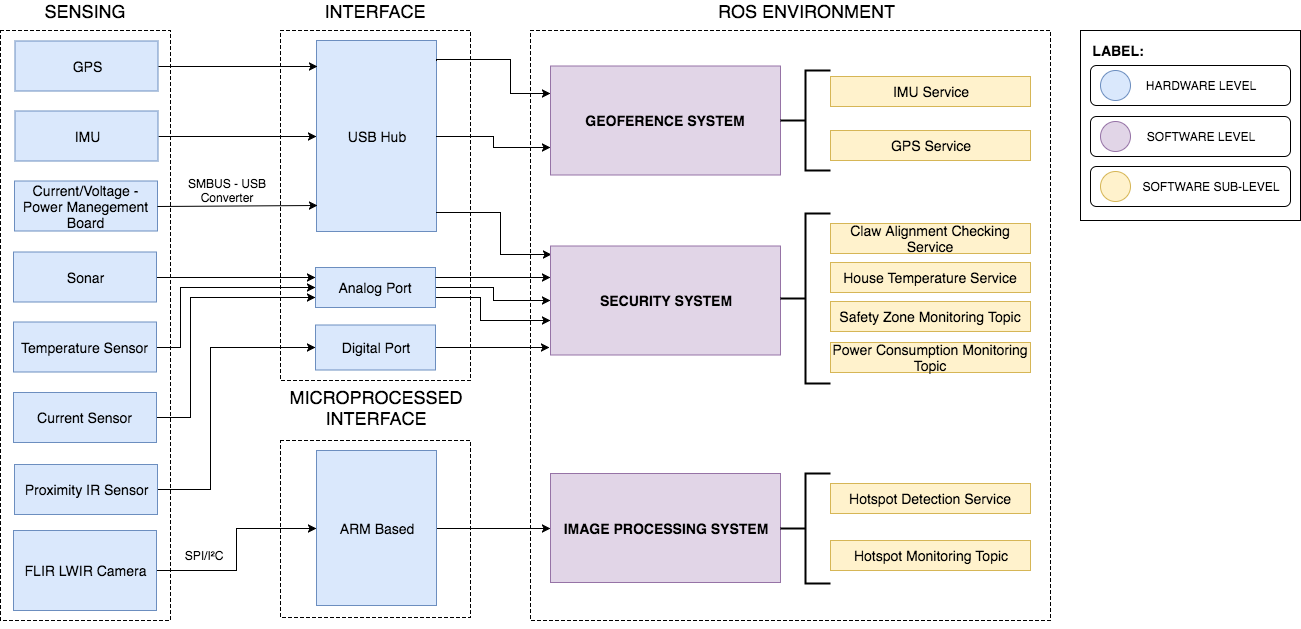
\includegraphics[width=15cm]{Figures/ArquiteturaPerceptionv2.png}
\caption{Arquitetura Geral da Perception}\label{arqgeral}
\end{figure}

 A etapa de Sensing é composta por todos os processos de aquisição de dados de todos os sensores envolvidos no projeto. A camada de interface compreende a disponibilização destes dados para o ambiente de trabalho ROS. Essas duas etapas são camadas de 0000000000hardware. Por último, terá a camada de software, a qual será feita no ROS Enviroment, e que irá englobar todo o sistema de compreensão e interpretação dos dados provenientes do sistema de interfaceamento do robô.
 
\subsection{Arquitetura de software}

A arquitetura de software foi projetada em três camadas a fim de facilitar o desenvolvimento do sistema e simplificar o entendimento do mesmo. As camadas de software são:

\begin{itemize}
\item User Interface Layer
\item Business Layer
\item Driver Layer
\end{itemize} 
As camadas e seus componentes podem ser vistos na Fig.\ref{arqsoft}.
\begin{figure}[H]
\centering
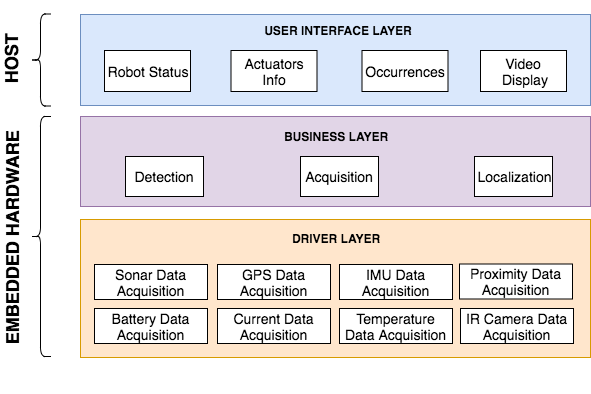
\includegraphics[width=15cm]{Figures/ArquiteturadeSoftware.png}
\caption{Arquitetura Geral da Perception}\label{arqsoft}
\end{figure}

\subsubsection{Driver Layer}
A camada de Driver Layer está diretamente relacionada a funcionalidade de aquisição de dados. Ela composta por partes físicas representadas pelos sensores e seus respectivos drivers de comunicação. Desta forma, as subcamadas são nomeadas com o processo de aqusição de dados de cada sensor envolvido no projeto.

As subcamadas \textit{Current Data Acquisition}, \textit{Temperatura Data Acquisition}, \textit{Proximity Data Acquisition} e \textit{Sonar Data Acquisition} são responsáveis por adquirir as informações analógicas de seus sensores e transformá-los em dados da grandeza física a ser medida. Todas estas subcamadas utilizam a placa de interfaceamento Phidgets para o estabeler de comunicação entre a NUC e os sensores.

As subcamadas \textit{IMU Data Acquisition} e \textit{GPS Data Acquisition} são responsáveis pelo recebimento de dados da IMU e do GPS seguindo o protocolo de comunicação do fabricante. 

A subcamada de \textit{IR Camera Data Acquisition} é responsável pela aquisição de dados da câmera térmica. 
Por último, a subcamada de \textit{Battery Data Acquisition} é responsável pelo estabelecimento da comunicação e coleta de informações com a placa multiplexadora de bateria utilizando protocolo I2C.

\subsubsection{Business Layer}

A camada de business layer é responsável por implementar a regra de negócio do sistema. A sub-camada management é quem realiza o processo de gerenciamento e controle das funcionalidades e por isso é representada com nível hierárquico maior do que as demais sub-camadas. As funcionalidades do sistema são representadas como sub-camadas da business layer pois ela são responsáveis pelo processamento e coordenação de dados adquiridos pela camada de aquisição. 


\subsubsection{User Interface Layer}

A camada de User Interface foi projetada para facilitar a interação com o usuário final. Ela tem o objetivo de disponibilizar de forma simplificada os dados mais relevantes do robô. Nesta camada existem três subcamadas: Robot Status Display, Actuators Display e Video Display. A subcamada Robot Status Display disponibiliza os dados de integridade do robô como temperatura, corrente, tensão, nível de bateria, entre outras informações. A subcamada de Actuators Display, disponibiliza o dados de todos os motores do robô, como carga, temperatura, status e corrente, desta forma o usuário pode acompanhar o desenvolvimento de todas as suas atividades. Por último, a subcamada de Video Display mostra em tempo real o monitoramento realizado pela câmera infravermelho e estéreo possibilitando o usuário de ver os componentes da linha que estão com temperatura elevada e até mesmo identificar pontos quentes, assim como verificar a imagem no plano RGB.

A interface irá se resumir em duas telas: A tela principal com um layout de dashboard, e outra que será as informações dos atuadores. O dashboard será um painel de monitoramento, no qual haverá as informações mais importantes da missão, como pode ser visto na Fig. \ref{UI} no apêndice D. Essa tela, além de monstrar as informações, irá pode dar o comando de início e parada da missão a partir dos botões "Start" e "Stop". A tela dos atuadores irá mostrar de forma organizada, as informações que foram mencionadas, além da corrente total de cada HUB de motores. Pode-se observar a tela de atuadores na Fig. \ref{UI2} no apêndice D.

\label{ssec:arqs}

%--------- NEW SECTION ----------------------
%\section{Desdobramento da função qualidade}
%\label{sec:qfd}
%asdfsdafsf

\subsection{Requisitos técnicos}
\label{ssec:reqt}
asdfsadfdsf


    \chapter{Materiais e Métodos}
\label{chap:mat}
asdfasdfsdf

%--------- NEW SECTION ----------------------
\section{Lista de componentes}
\label{sec:espc}
%\subsection{Estrutura analítica do protótipo}
%\label{ssec:pbs}
%asdkjfsdalkjf
Para a confeção do sistema de percepção foi necessário a aquisição dos seguintes itens:
\begin{table}[]
\centering
\begin{tabular}{|l|l|l|l|}
\hline
{Item}                           & {Qtd.} & {Preço Unit.} & {Preço Total}  \\ \hline
Phidgets Interface Kit 8/8/8     & 1  & R\$ 271,82  & R\$ 271,82  \\ \hline
Nucleo STM32F401RE               & 1  & R\$ 43,287  & R\$ 43,287  \\ \hline
Sensor de Proximidade BCBI5770   & 5  & R\$ 36,90   & R\$ 184,50  \\ \hline
Maz-Sonar EZ1                    & 1  & R\$ 101,76  & R\$ 101,76  \\ \hline
IMU XSENS MTi 1                  & 1  & R\$ 1597,5  & R\$ 1597,5  \\ \hline
GPS Swiftnav Piksi 1.3.2         & 1  & R\$ 3398,0  & R\$ 3398,0  \\ \hline
Sensor de Temperatura LM35       & 1  & R\$ 5,75    & R\$ 5,75    \\ \hline
Câmera LWIR Lepton FLIR          & 1  & R\$ 812,05  & R\$ 812,05  \\ \hline
Phidgets Current Sensor          & 3  & R\$ 105,329 & R\$ 315,98  \\ \hline
NUC5i5RYK                        & 1  & R\$ 1380,83 & R\$ 1380,83 \\ \hline
Smart Charger EB325A             & 1  & R\$ 2200,00 & R\$ 2200,00 \\ \hline
Placa de Gerenciamento de Energia & 1 & R\$ 1004,16 & R\$ 1004,16 \\ \hline
Baterias DSNH2054HD34            & 2  & R\$ 1004,16 & R\$ 2008,32 \\ \hline
Nucleo STM32L432KC                      & 1  & R\$ 20,20   & R\$ 20,20   \\ \hline
\end{tabular}

\caption{Lista de Componentes}
\end{table}
\pagebreak
Todos os itens já estavam disponíveis para uso na área de robótica. A única excessão foram os sensores de proximidade, os quais tiveram que ser comprados.



%--------- NEW SECTION ----------------------
\section{Diagramas mecânicos}
\label{sec:diagm}

\subsection{Suportes para os componentes internos do robô}

Para fixar todos os sensores e componentes eletrônicos de maneira organizada, foi desenhado uma estrutura em forma de prateleira, na qual é possível anexa-los. As peças foram impressas em uma impressora 3D de forma que seja possível encaixa-las uma nas outras para facilitar o desenvolvimento. Essa peça irá ficar no compartimento superior da housing do robô.

Na Fig. \ref{Prateleira} é possível observar três peças empilhadas e na Fig. \ref{Prateleiracsensor} se vê a mesma com os sensores presos.

    \begin{figure}[H]
	\centering
	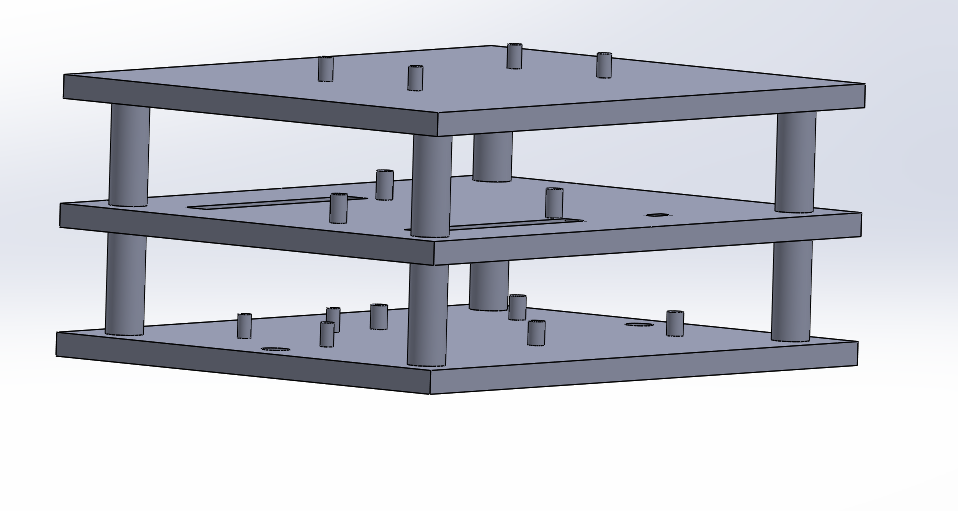
\includegraphics[width=14cm]{Figures/prateleira.png}
	\caption{Prateleira para suporte dos componentes eletrônicos} \label{Prateleira}
	\end{figure}
	
	\begin{figure}[H]
	\centering
	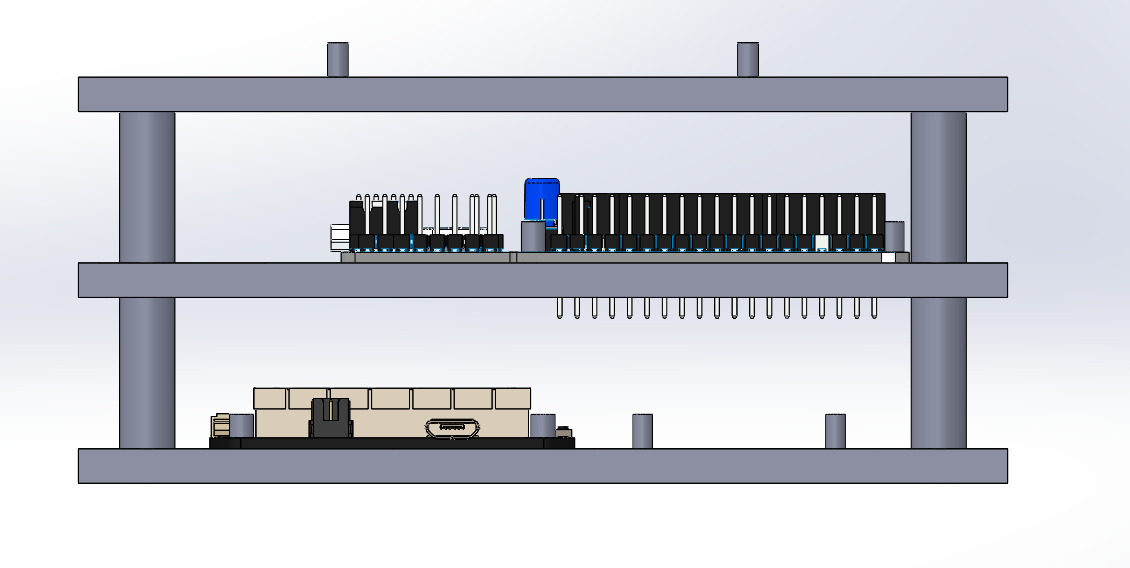
\includegraphics[width=16cm]{Figures/prateleiracsensores.png}
	\caption{Prateleira para suporte com sensores} \label{Prateleiracsensor}
	\end{figure}

O compartimento inferior da housing será utilizada para os componentes relacionados a energização do robô. Isso inclui as baterias, carregador inteligente e a placa de gerenciamento de energia. Para a fixação desses componentes foi desenvolvida a seguinta peça.

	\begin{figure}[H]
	\centering
	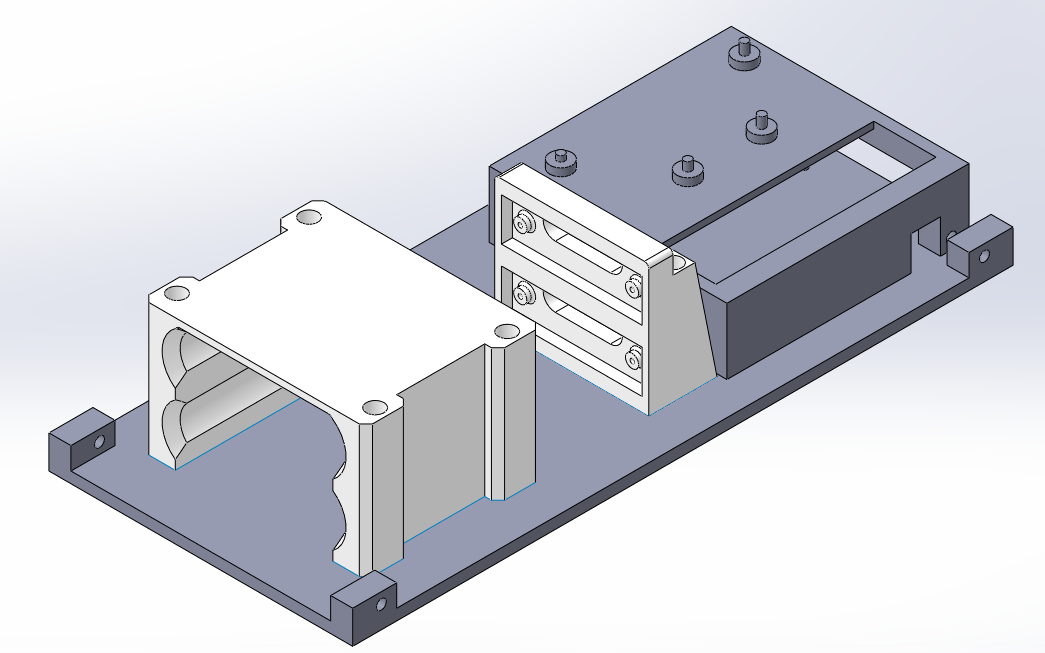
\includegraphics[width=14cm]{Figures/pecadebaixo.png}
	\caption{Prateleira para suporte dos componentes de alimentação} \label{pecaaliment}
	\end{figure}
	
	Todos os componentes serão fixados na estrutura do robô sem realizar nenhum furo ou alteração na mesma.
%--------- NEW SECTION ----------------------
\section{Modelo esquemático de alimentação e comunicação}
\label{sec:modesq}

A alimentação do sistema é proveniente de duas baterias LiPo que fornecem tensão de 14V. Todo o gerenciamento de energia do sistema é feita pela Power Management Board, esta placa é responsável por distribuir a alimentação de entrada para os demais subsistemas da Perception. 

A placa de interface Phidgets além de funcionar como hub para uma grande parte dos sensores também é responsável por compatibilizar o nível de tensão para os equipamentos eletrônicos, fornecendo 5V para as placas microprocessadas, sensores e a alimentação de todas as USBs. 

A comunicação entre os sistemas da Perception na maior parte acontecem através da Phidgets, já que ela concentra as informações uriundas de suas portas USB, entrada digitais e entradas analógicas em uma única porta USB para a NUC. Porém, a câmera térmica e a comunicação com os dynamixels acontecem de forma independente. Estes possuem portas USBs dedicadas na NUC.

O esquemático de alimentação e comunicação entre todos os elementos do sistema de Percepção está disponibilizado no apêndice XX.

\subsection{Diagramas elétricos}
\label{sec:diage}
O diagrama elétrico do sistema está disponível no apêndice XX. Neste diagrama encontram-se todas as conexões elétricas e de comunicação bem como as especificações de conectores e cabos utilizados no projeto. 

\subsection{Esquemas eletrônicos}
\label{ssec:esqe}

O único esquemático eletrônico realizado pela equipe da Perception foi uma placa hub de 5V para poder alimentar os sensores de proximidade visto que a Phidgets possui apenas umas saída de 5V disponibilizada. Nesta placa foram colocados os pin header para cada sensor de proximidade, fornecendo 5V, GND e os pinos digitais dos sensores foram disponibilizados em um conector Molex para facilitar o cabeamento entre o hub e a Phidgets.

O esquemático eletrônico e board estão mostrados no anexo XX.

%--------- NEW SECTION ----------------------
\section{Especificação das funcionalidades}
\label{sec:espf}
asdfadsfsdfs

%\subsection{Fluxo das informações}
%\label{ssec:fluxo}
%asdfsaf

\subsection{Aquisição}
\label{ssec:func1}
    \subsubsection{Objetivo}
    Realizar a comunicação e a aquisição dos dados provinientes da câmera térmica, sensores de proximidade, sonar, GPS, IMU, sensor de temperatura, placa multiplexadora de bateria e sensores de corrente.
        
     \subsubsection{Dependências}
     Esta funcionalidade não é dependente de nenhum outro processo.
    
     \subsubsection{Premissas}
     	\begin{itemize}
        	\item A interface microcontrolada Nucleo STM32F401RE deve estar com firmware embarcado para conversão de dados SPI para UART.
            \item A câmera térmica deverá estar conectada à interface Nucleo STM32F401RE
            \item A câmera stereo deve está conectada à NUC através da porta USB
            \item O sensores de temperatura, corrente e sonar devem estar conectados as entradas analógicas da interface Phidgets
            \item O sensor de proximidade deve está conectado a entrada digital da interface Phidgets
            \item O GPS e a IMU devem estar conectados a portas USB da Phidgets
            \item As placas de interface devem estar energizadas.
        \end{itemize}
     
     \subsubsection{Descrição da Funcionalidade}
        	 \indent O processo de aquisição de dados envolve a comunicação dos sensores com seus respectivos drivers no ambiente ROS e a disponibilização dos dados para as outras funcionalidades do sistema.\\
     \indent Os sensores analógicos e digitais terão seus dados tratados pelo driver da interface Phidgets no ambiente ROS.\\
     \indent Para os dispositivos relacionados a localização como o GPS e a IMU, será utilizado drivers já disponibilizados pela comunidade do ROS, os dados desses drivers serão recebidos por um \textit{package} que unirá os dados de localização em uma única menssagem.\\
     \indent Os sensores que necessitam de um protocolo de comunicação SPI ou I2C, como a câmera térmica e a placa multiplexadora de baterias, será utilizado duas interfaces baseadas em ARM com um \textit{firmware} embarcado para a conversão dos dados para o protocolo USB para serem conectados a unidade de processamento Intel NUC. No ambiente ROS terá um driver para receber os dados convertidos da câmera térmica, assim como um driver para receber os dados da multiplexadora de baterias e da câmera stereo.
     Pode-se observar o fluxograma da aquisição na Fig. \ref{FuncAquisition}
     
    \begin{figure}[!ht]
	\centering
	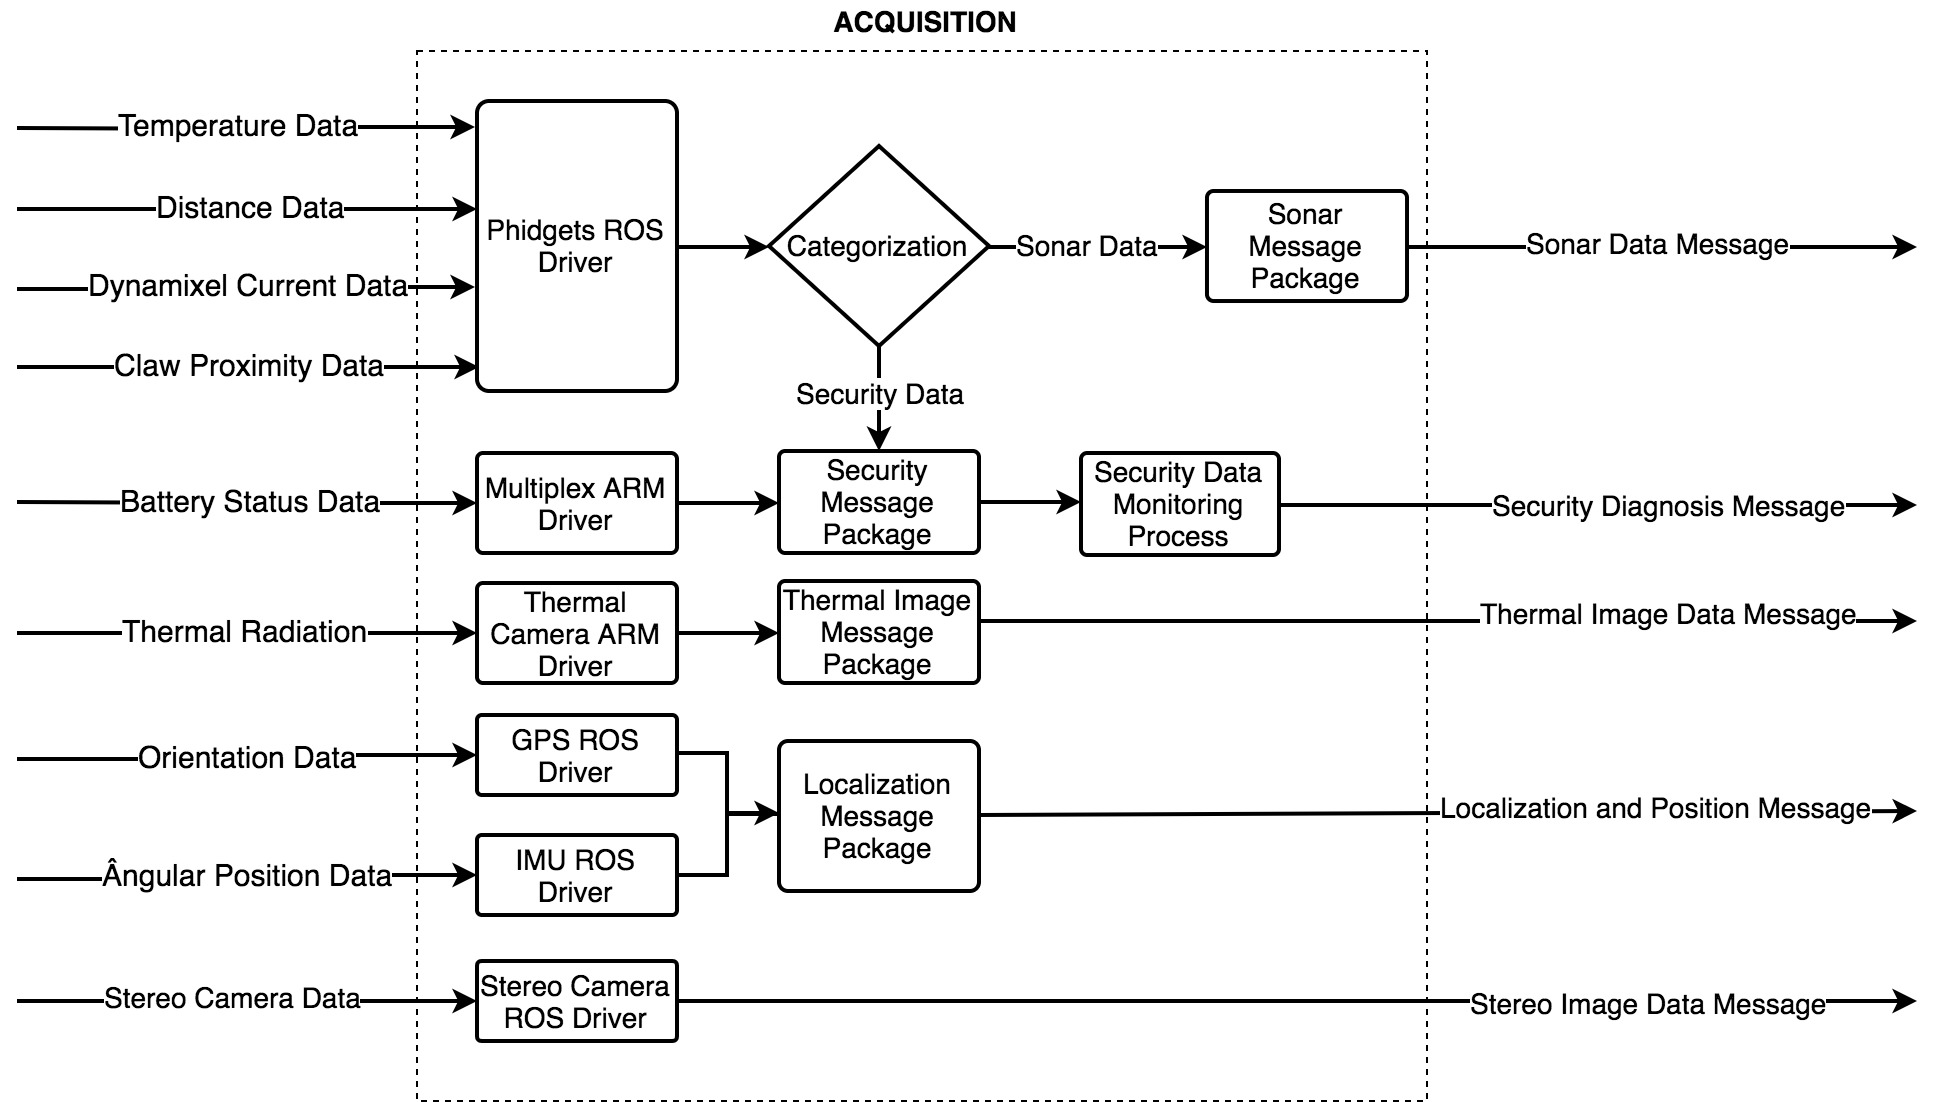
\includegraphics[height=7cm, width=14cm]{Fluxograma_Aquisition.jpg}
	\caption{Fluxograma da Funcionalidade Aquisição} \label{FuncAquisition}
	\end{figure}
	
      Para correta execução desta funcionalidade é necessário o funcionamento dos sensores segundo o nível de prioridade dos mesmos. Logo, um estudo de casos de falhas para cada sensor foi realizado, no qual foi definido um nível de criticidade de acordo com o impacto de sua função no sistema como um todo. Foram elaborados três níveis de criticidade:
     \begin{itemize}
     	\item Level 1 - Sensores com impacto crítico na operação. Em casos de falha, a inspeção não poderá ser realizada.
        \item Level 2 - Sensores com impacto médio na operação. Em caso de falha, a inspeção poderá ser realizada de forma parcial.
        \item Level 3 - Sensores com impacto leve na operação. Em caso de falha, não haverá dados de monitoramento da situação de temperatura e consuno energético do robô, porém a inspeção poderá continuar normalmente.
	\end{itemize}
	
	Na figura abaixo, pode-se observar os sensores e suas categorias.
	
	\begin{figure}[!ht]
	\centering
	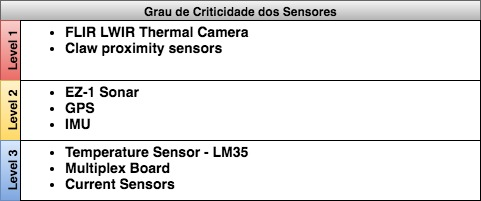
\includegraphics[height=7cm, width=14cm]{Figures/criticidade.jpg}
	\caption{Nível de criticidade dos sensores} \label{FuncAquisition}
	\end{figure}
	
	\subsubsection{Saídas}
     
     Esta funcionalidade possui quatro saídas:
     
    \begin{itemize}
        	\item Sonar Data Message: Mensagem de saída exclusiva para os dados do sonar EZ-1.
            \item Secutiry Diagnose Message: Mensagem contendo todos os dados relacionados à segurança e integridade do robô.
            \item Thermal Image Data Message: Mensagem exclusiva para os dados da câmera térmica.
            \item Localization and Position Message: Mensagem contendo os dados relacionados á localização e posicionamento angular do robô.
            \item Stereo Image Data Message: Mensagem exclusiva para os dados da câmera stereo.
        \end{itemize}
\pagebreak
\subsection{Localização}
\label{ssec:func2}
    \subsubsection{Objetivo}
        O objetivo desta funcionalidade é disponibilizar os dados de Localização do robô no ambiente ROS para a funcionalidade de Detecção.

    \subsubsection{Dependências}
        O sistema de localização depende dos dados de posicionamento e orientação disponibilizados pelo sistema de Aquisição.

    \subsubsection{Premissas}
        \begin{itemize}
         	\item O sistema de Aquisição deve está funcionando corretamente até o Nível 2 de criticidade dos sensores.
             \item GPS e IMU estão posicionados em uma estrutura rígida e com o menor vibração possível.
        \end{itemize}
        
    \subsubsection{Descrição da Funcionalidade}
        O sistema de localização envolve o monitoramento da posição latitudinal e longitudinal do robô, assim como a posição angular através do GPS e da IMU respectivamente.
        
        A localização é um package que ao receber uma requisição de informação, coleta os dados de posicionamento e orientação do robô provenientes do sistema de Aquisição e encaminha para o sistem que requisitou.
        
        O fluxograma deste funcionalidade pode ser visto na Figura \ref{fluxlocal}

        \begin{figure}[h!]
        	\centering
        	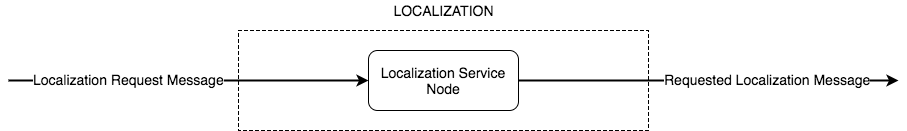
\includegraphics[width=16cm]{Fluxograma_Localization.png}
        	\caption{Fluxograma da Funcionalidade Localização} \label{fluxlocal}
    	\end{figure}
        \pagebreak
    \subsubsection{Saídas}

    \begin{itemize}
        	\item Requested Localization Message: Mensagem que informa os dados de localização para o sistema que os requisitou.
    \end{itemize}

    \subsection{Detecção}
\label{ssec:func3}

\subsubsection{Objetivo}

O objetivo desta funcionalidade é coletar as informações provinientes da câmera infravermelha e do sonar, como detectar a presença de pontos quentes e objetos presentes na área de servidão. Caso algum destes seja detectado, será enviado uma mensagem de alerta .

\subsubsection{Dependências}
 O sistema de detecção depende dos dados do sonar, frames da câmera térmica e frames da câmera stereo disponibilizados pelo sistema de Aquisição. Além disto, depende do sistema de Localização para adquirir informações de posicionamento e orientação do robô.

\subsubsection{Premissas}
\begin{itemize}
        	\item O sistema de Aquisição deve está funcionando corretamente até o Nível 2 de criticidade dos sensores.
            \item A câmera térmica deve estar calibrada e posicionada com ângulo de visão para as linhas de transmissão e seus obstáculos
            \item A câmera stereo deve está calibrada e posicionada com visada direta para os obstáculos.
            \item O sonar deve estar posicionado de forma a monitorar objetos abaixo da linha de transmissão.            
\end{itemize}

\subsubsection{Descrição da Funcionalidade}

A detecção é a funcionalidade responsável por identificar a presença de pontos quentes na linha de transmissão bem como de objetos na faixa de servidão. Ao identificar um destes elementos, o sistema solicita da funcionalidade de Localização os dados posicionamento e orientação do robô e envia uma mensagem de alerta.

A mensagem de alerta da detecção de um ponto quente informa a localização do robô e a localização do objeto no frame de imagem. Por isso recebe a mensagem de detecção de obstáculos. O package compara a região no frame de imagem da câmera stereo que contém o obstáculo com o frame da câmera IR com informação de ponto quente. 

A mensagem de detecção de objetos na faixa de servidão informa a distância da cota da linha até o objeto e a localização do mesmo. 

    \begin{figure}[!ht]
	\centering
	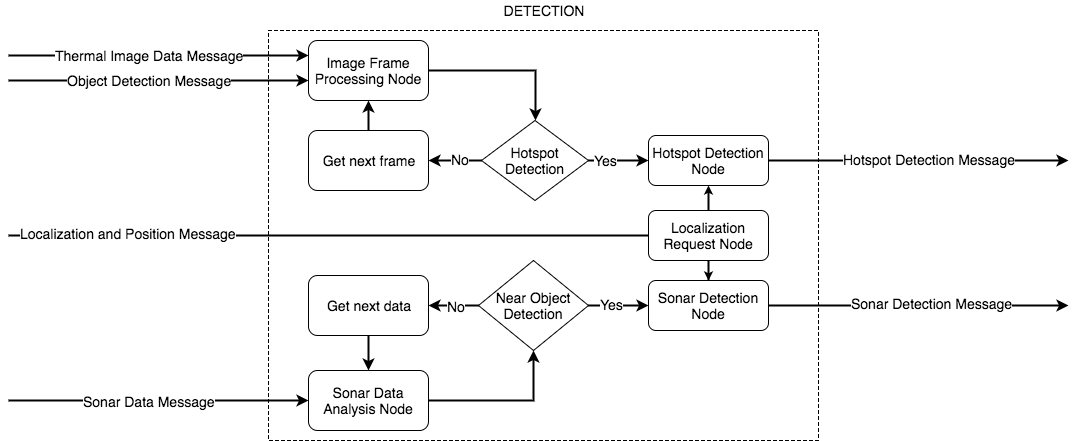
\includegraphics[width=16cm]{Fluxograma_Detection.png}
	\caption{Fluxograma da Funcionalidade Detecção} \label{FuncDetec}
	\end{figure}

\subsubsection{Saídas}

    \begin{itemize}
        	\item Hotspot Detection Message: Mensagem que informa a detecção de um ponto quente e informa a sua localização na imagem e localização do robô na linha.
            \item Sonar Detection Message: Mensagem que informa a detecção de objetos na faixa de servidão e sua localização na linha.
            %\item Localization Request Message: Mensagem de requisição dos dados posicionamento e orientação do robô para o sistema de Localização
    \end{itemize}
    \pagebreak

%--------- NEW SECTION ----------------------
\section{Interface do Usuário}
\label{sec:ui}
    \begin{figure}[!ht]
	\centering
	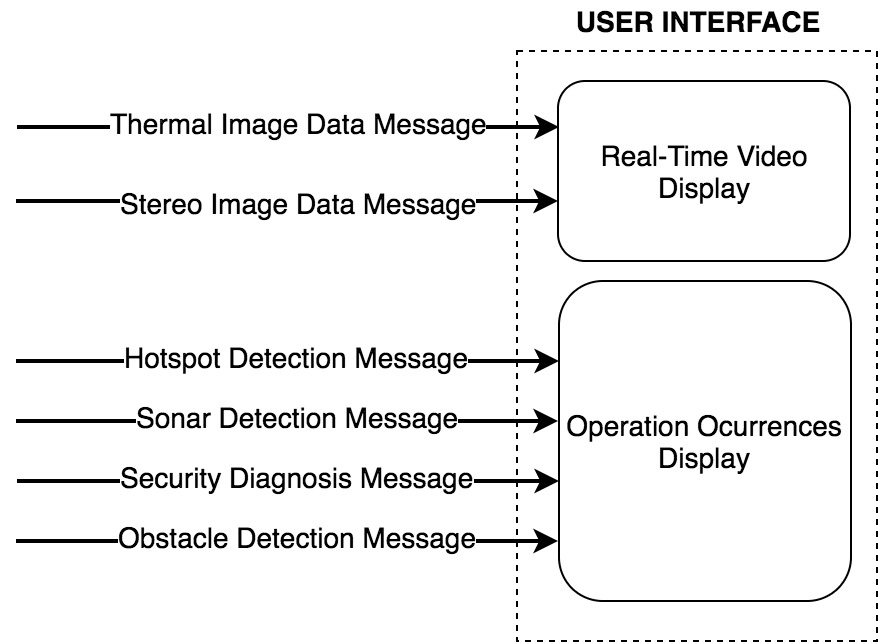
\includegraphics[width=16cm]{Figures/Fluxograma_Interface.jpg}
	\caption{Fluxograma da Interface do Usuário} \label{UI}
	\end{figure}
	


\pagebreak
\newpage
%--------- NEW SECTION ----------------------
%\section{Simulação do sistema}
%\label{sec:sim}
%asdfadsfsdfs



    \chapter{Resultados}
\label{chap:result}

As funcionalidades do sistema de percepção foram validades a partir de duas etapas de teste. Os testes unitários buscam a validação do funcionamento de cada sensor individualmente enquanto os testes integrados validam o funcionamento dos sistemas e funcionalidades. A descição dos testes realizados e dos resultados obtidos por eles está descrita abaixo.

%--------- NEW SECTION ----------------------
\section{Testes unitários}
\label{sec:testu}

    \subsection{Câmera Térmica}
    
    A câmera térmica se comunica por VOSPI. Logo, foi necessário utilzar um driver para converter os dados da câmera e disponibilizá-los para USB. Foi utilizada a placa de interface Nucleo STM32F401RE com o driver disponibilizado por \citeonline{groupgets}. 
    
    O driver apenas coleta os frames e envia para a USB seguindo o seguinte padrão de mensagem:
    
    \begin{figure}[!ht]
    	\centering
    	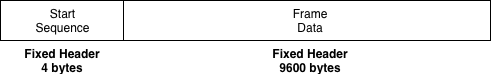
\includegraphics[width=14cm]{Figures/frame_msg.png}
    	\caption{Mensagem do frame da câmera} \label{framemsg}
	\end{figure}
    
    Na qual cada \textit{pixel}, dois \textit{bytes}, foi convertido para uma escala de cinza de 8-bit através de um algoritmo em python no computador, necessária para trabalhar com a biblioteca de processamento de imagens OpenCV.
    
    Após isso a imagem era reconstruida para verificar o funcionamento da câmera.
    
    \subsection{Sonar EZ-1}
    O sonar EZ-1 da MaxBotix possui saída analógica, desta forma para cada distância medida existe um valor de tensão associado no pino AN do sonar. Para testar o sensor de proximidade foi utilizada uma das portas analógicas da Phidgets que possui um pino de VCC, um de GND e um pino Analógico. Com o driver da phidgets instalado no computador e funcionando foi necessário apenas conectar os pinos de VCC, GND E AN do sensor nos pinos correspondentes da Phidgets e compilar um código para leitura de tensão - disponibilizado no próprio site da Phidgets - no terminal do computador. 
    
    Ao compilar o código você recebe no intervalo de 10s todas as leituras de tensão efetuadas no sensor. Notamos que ao afastar o obstáculo do sonar o valor de tensão aumentava e quando aproximavamos o obstáculo o valor de tensão diminuia, indicando a linearidade do sensor e validando o seu funcionamento.
    
    \subsection{Sensor de Proximidade}
    O sensor de proximidade possui um LED vermelho em sua estrutura, toda vez que o sensor identifica a presença de algum objetivo o LED ascende. Por isso, o sensor foi alimentado através de uma fonte de tensão ajustada para 5V e o LED foi observado. Ao colocar um objeto na frente do sensor a luz ascendia e ao retirar o objeto a luz apagava, indicando o pleno funcionamento do sensor.
    
    \subsection{Sensor de corrente}
    
    O sensor de corrente da Phidgets consegue ler valores entre -30 a +30 com resolução de 75mA. Por isso para testar do sensor era necessário uma fonte de corrente com valor maior que 75mA. O circuito utilizado para fornecer essa corrente foi um LED de alto brilho com um resistor de potência em série. A corrente estimada foi de 100mA. Para testar o funcionamento do sensor este precisava ter seus dois canais de entrada conectados em série no circuito e a saída do mesmo foi conectado na porta analógica da Phidgets. A partir do script VoltageInput anteriormente mencionado, foi possível obter os dados de corrente da leitura do sensor. Os dados obtidos foram compatíveis com os valores de corrente real confirmando o funcionamento do sensor. 
    

    \subsection{Smart Charger}
    
    A placa de gerenciamento e carregamento das baterias funciona a partir do protocolo de comunicação SMBus, este protocolo é baseado no protocolo i2c. As informações de tempertatura, tensão, carga entre outras possuem uma codificação. Por isso para comunicar com a placa você precisa escrever uma mensagem para ela contendo o endereço da bateria que você quer ler a informação, o código da informação que você quer ler e entrar com o endereço de memória no qual a informação será escrita.
    
    Foi implementado um código na placa de interface Nucleo STM32L432 para receber as informações provenientes da Smart Charger e disponibiliza-la na USB da placa. Foram lidos os dados de temperatura, carga e tensão. Os dados obtidos foram convertidos para valores em grau celsius, KWh e Volts respectivamente e assim puderam ser validados. 

    \subsection{Sensor de Temperatura }
    
    O sensor de temperatura LM35 é um sensor com saída analógica e com comportamento linear entre a tensão de saída e a temperatura medida. O sensor foi testado em uma das portas analógicas da Phidgets, conectando os pinos de VCC,GND E AN do sensor nos pinos correspondentes na Phidgets e o algoritmo de leitura de tensão foi utilizado para realizar a obtenção de dados. Para simular ambientes quentes e frios, foi medido o valor de tensão de saída para uma sala com ar-condicionado e após isto foi medido a temperatura assoprando o sensor. O valor da tensão de saída aumentou, como o sensor é linear e o valor de temperatura é o valor da tensao de saída multiplixado por 10, foi possível confirmar a coerência dos valores encontrados validando o funcionamento do sensor.
    \subsection{GPS}
    
    O GPS foi testado a partir de um console disponibilizado no próprio site do fabricante. Foi necessário instalar esse console e conectar o GPS na USB do computador. A sua antena também foi acoplada. Como os dados do GPS só são confiáveis quando existem pelo menos 4 satélites conectados e a recepção na sala de teste era rui, no próprio console foi colocado o GPS no modo de simulação. A interface foi simples e assim que o console foi aberto foi colocada a taxa de dados de 15200 bauds. Após isso uma outra tela foi aberta informando os dados de latitude e longitude lidos. 
    
    \subsection{IMU}
    
    A IMU Xsens Mti-1 series possui um console chamado MtManagement e que é disponibilizado no próprio pen-drive de instalação que vem junto ao sensor. O console foi instalado e foi necessário apenas conectar a IMU a uma das portas USB do computador. Na própria interface gráfica já aparece as informações de orientação do dispositivo, informando a orientação nos três eixos de referência e velocidade angular. 
    
    \subsection{Phidgets}
    
    A phidgets é uma placa de interface com vários periféricos. Para testar as portas USBs presentes na placa foi conectado um pen drive na porta USB da Phidgets e a mesma foi conectada a uma porta USB do computador. O dispositivo foi acesso normalmente pelo computador indicando que a função da Phidgets de hub USB funcionou perfeitamente.
    
    Para obter dados das portas analógicas e digitais da phidgets é necessário o download e instação da biblioteca LibPhidget22 e do python module. Estes estão disponibilizados no próprio site da Phidgets com todas as intruções de instalação e exemplos de testes. Após a instalação da biblioteca foi o utilizado o exemplo de código VoltageInput.py e DigitalInput.py do site da Phidgets para se comunicar com os sensores conectados as portas. Ao compilar o código no terminal do computador foram adquiridos os dados dos sensores acoplhados a Phidgets indicando o funcionamento de suas portas.
    
     \section{Integração no ROS}
     
     Após os testes unitários de cada sensor foi necessário o embarque no ambiente ROS para construção do sistem de Percepção. A descrição da metodologia empregada para embarcar cada um dos sensores no framework de robótica está mostrada nos tópicos abaixo.
     \subsection{Phidgets}
     A Phidgets por ser uma placa de interface concentra dispositivos que se comunicam de forma analógica e digital, por isso foi criado em ambiente ROS um nó responsável por coletar informações dos dispositivos conectados a Phidgets. O nó foi criado através de funções presentes na biblioteca da Phidgets e tendo como exemplo o algoritmo VoltaInput.py comentado anteriormente. 
     
     O nó foi construído utilizando a linguagem python e consiste em uma classe, cada dispositivo conectado a Phidgets corresponde a um objeto da classe criada onde são definidos a porta a qual o dispositivo está conectado, o tipo de comunicação (digital ou analógico), o nome do sensor e o nome do tópico a ser publicado as informações dos sensores. Após a criação dos objetos da classe é necessário chamar o método setup() de cada objeto para obter a tensão na porta dos sensores analógicos ou o estado da porta no caso dos sensores digitais. As informações são publicadas nos tópicos criados através de um método Publisher característico do ROS.
     
     Os sensores digitais conectados as portas da Phidgets foram os sensores de proximidade, enquanto que o sensor analógico conectado a Phidgets foi o sonar. O scrip desenvolvido como nó para  Phidgets está mostrado no Anexo XX.
     
     \subsection{Smart Charger}
     
     O script utilizado no teste unitário para receber os dados provenientes da smart charger no computador foi utilizado como base para a construção do nó no ambiente ROS. O script funciona enviando o caracter '0' via Serial o que faz a placa de interface Nucleo conectada a Smart Charger retornar todas as informações necessárias da bateria. No nó do ROS essas informações são recebidas via Serial, colocadas em um formato de mensagem chamado de Battery e publicadas em um tópico do ROS. O nó criado para a Smart charger está mostrado no anexo XX.
     
     \subsection{Câmera Térmica}
     
     A integração da câmera no ROS foi feita em duas etapas, que na prática foram representadas como dois nós:
     
     \begin{itemize}
         \item O primeiro com objetivo da aquisição dos dados da câmera e sua disponibilização em um tópico.
         \item O segundo nó é responsável por todo o tratamento da imagem e detecção dos pontos quentes.
     \end{itemize}
     
     Para a aquisição dos dados, no primeiro nó, foi utilizado basicamente o mesmo algoritmo que no teste unitário, porém com a integração das bibliotecas do ROS.
     
     No segundo nó foi utilizado a biblioteca OpenCV para realizar o processamento da imagem. Primeiramente, o frame disponibilizado pelo nó de aquisição é adquirido subscrevendo do seu respectivo tópico. Para retirar o aspecto "pixelado" da imagem da câmera, devido a sua baixa resolução (80x60 pixeis), foi necessário realizar uma interpolação cúbica para redimensionar a imagem para uma resolução de (400x300 pixeis), obtendo assim uma imagem mais detalhada. 
     
     Com a imagem já redimensionada, é aplicado um filtro \textit{blur} para eliminar altas frequências que podem interferir na binarização (\textit{thresholding}) que será feita na imagem.
     
     Após o filtro, o frame é binarizado com o objetivo de facilitar a identificação dos pontos quentes através de um algoritmo de busca de contornos.
     
     \subsection{GPS}
     
     Foi utilizado um driver disponibilizado no GitHub com licença livre para embarcar o GPS no ambiente ROS. O driver pertence a xxxx. 
     
     \subsection{IMU}
    Foi utilizado o driver da IMU disponibilizada pela própria fabricante Xsens para embarcar a IMU no ROS. O driver de licença livre é disponibilizado no github da própria empresa. 
    
%--------- NEW SECTION ----------------------
%\section{Testes integrados}
%\label{sec:testi}
%asdfadsfsdfs

%--------- NEW SECTION ----------------------
%\section{Avaliação da prontidão tecnológica}
%\label{sec:trl}
%asdfadsfsdfs

%--------- NEW SECTION ----------------------
%\section{Trabalhos futuros}
%\label{sec:trabfut}
%asdfadsfsdfs






    %\chapter{Título do capítulo}\label{chapter:outro}

As organizações atuam em um ambiente global altamente competitivo, dinâmico, complexo e instável. Tais características denotam cenários de imprevisibilidade, onde todas as suas operações e atividades precisam ser vistas e revistas continuamente. Neste contexto do mundo dos negócios, é de fundamental importância que as organizações busquem estratégias eficazes para suas operações - planejamento, marketing, finanças, produção, qualidade e a logística - por serem cada vez mais importantes e por estarem relacionadas diretamente com as atividades fim dos variados sistemas produtivos.

Busca-se, portanto, reduzir custos em toda cadeia de valor e prover a satisfação dos clientes. Por esta ótica é possível entender o porquê da logística está em evidência na conjuntura atual de mercado. O fato desta ser amparada nos pilares: transportes, gestão de estoques, processamento de pedidos, atividades de apoio e ter como objetivo prover o cliente com os níveis de satisfação desejados pelos mesmos, faz com que a logística assuma um papel fundamental para as organizações: ser um componente capaz de gerar uma vantagem competitiva fundamental, ou seja, providenciar bens e serviços de maneira correta, em tempos e lugares exatos, na condição desejada e em menor custo possível.

Entretanto, quando se fala em melhoria da eficiência operacional na distribuição física, não é suficiente considerar apenas o meio de transporte mais utilizado no Brasil - o rodoviário; é preciso, analisar toda matriz de transporte disponível, para alcançar um serviço capaz de atender satisfatoriamente o canal de vendas. Essa visão considera cada etapa do processo de transporte, procurando sempre identificar as possíveis alternativas, muitas vezes descartadas ou mal exploradas.

Conforme Lambert, Stock e Vantine (1998), estima-se que no Brasil os gastos com atividades logísticas correspondam a 17\% do Produto Interno Bruto (PIB) e, na média, o transporte envolve 60\% dos custos logísticos das empresas. Estes dados justificam a necessidade de um sistema de transporte possuir mecanismos capazes de analisar quais opções de modais apresentam-se mais adequadas ao seu contexto de negócio. Ressalta-se ainda, que a seleção de modais afeta diretamente o preço dos produtos, as condições de entrega e a pontualidade, elementos estes considerados estratégicos para que o sistema alcance seu objetivo.

Segundo os mesmo autores, os cinco principais modais básicos são: rodoviário, ferroviário, aquaviário, dutoviário e aéreo, e sua importância relativa deve ser medida em termos de quilometragem do sistema, volume de tráfego, receita e natureza de composição. Justamente por tais questões que o modal aquaviário se configura como uma alternativa importante para a matriz de transportes brasileira, principalmente quando se fala em cabotagem, devido as características geográficas do Brasil.

Qualquer pesquisa efetuada no Brasil sobre modal aquaviário depara-se imediatamente com a seguinte questão fundamental: por que esse modal logístico é menos usado do que a lógica indicaria? O mesmo é verdade para o modal ferroviário. Por que são tão minguados face ao modal rodoviário? Qual a causa desse "transtorno dos modais", essa terrível modalidade de doença logística que aflige o Brasil e constitui uma de suas mais graves patologias?

Muitos estudos têm analisado essa síndrome de hipertrofia rodoviária e anemias ferroviária e aquaviária. Segundo a COPPEAD-UFRJ, o modal rodoviário responde por cerca de 60% de tudo que é transportado no país, enquanto em países de dimensões territoriais equivalentes ao Brasil, como os EUA e a Rússia, esses percentuais são, respectivamente, 35% e 19%.

Independentemente de comparações entre países, salta aos olhos imediatamente o absurdo de se transportar por caminhão cargas de São Paulo a Fortaleza ou Belém, em trajetos de mais de 3.000 km, quando existe a possibilidade de se usar a cabotagem, mais econômica e menos poluidora.

A considerável literatura técnica que versa sobre cabotagem refere-se quase exclusivamente à carga geral conteinerizada, porque é nessa área que reside o maior potencial de alteração de modal. Em matéria de granéis líquidos e sólidos, a maior parte do que pode ser transportado por cabotagem já o está sendo. Ademais, nesse caso, o transporte dutoviário é geralmente mais indicado.

As lamentações sobre a pouca utilização do modal de cabotagem devem ser entendidas como referentes sobretudo à submodalidade de carga geral. Mas há também absurdas quantidades de caminhões transportando granéis sólidos e líquidos a grandes distâncias nas estradas nacionais. A cabotagem, por sua vez, é parte de uma categoria mais ampla, o modal aquaviário ou hidroviário, dividido em dois submodais: cabotagem e transporte fluvial, esse chamado também de navegação interior, que envolve rios, canais e lagoas.

Portanto, pode-se afirmar que o processo de globalização, o transporte intermodal e as revoluções tecnológicas dos últimos anos na indústria de transporte fluvial resultaram em uma busca maior pela otimização das operações de empresas diretamente envolvidas nesse modal e, principalmente, na expansão das chamadas redes marítimas. No entanto, a falta de dados precisos sobre as relações entre os portos, vem impedindo uma maior aplicação da teoria de redes marítimas, que muitas vezes são analisadas por meio de estudos de caso de empresas ou regiões específicas.

A pesquisa e análise do referencial teórico especializado, na área de redes marítimas, demonstram que a grande maioria dos estudos e produção científica investigam pouco a resolução de problemas específicos sobre essas redes, especialmente observando importantes fatores diretamente relacionados a elas como movimentação de cargas, que interferem de maneira coordenada e agregadora no comportamento individual de cada nó dessa rede, ou seja, os portos.

Assim sendo, as análises de redes marítimas se constituem como um dos maiores campos a serem explorados pela evolução do conceito de redes sociais. Neste sentido, este projeto objetiva analisar a estrutura espacial e dinâmica regional da movimentação de contêineres por cabotagem entre os principais portos na costa brasileira, contribuindo com o estado da arte da seguinte maneira: (1) construindo e analisando redes marítimas, com a utilização de softwares especializados para modelagem computacional dessas; (2) hierarquizando os portos brasileiros através da metodologia AHP e (3) identificando possíveis formações de "clusters" entre os operadores logísticos envolvidos nessas redes através das chamadas constelações competitivas. O resultado da junção dessas análises poderá potencializar positivamente a cabotagem brasileira na obtenção de importantes impactos relacionados à sua gestão.

    %
\chapter{Scenario Definitions and Network Analysis}\label{chpdata}

This chapter illustrates the use of our model to represent a real world population,
summarises the model's options and examines the properties of the underlying small world
network representation for a variety of scenarios. It highlights and contrasts the
model's strengths and weaknesses as compared with the original small world model
\cite{Watts1998} and traditionally used social network models.


\section{Scenarios}

The data used to define the population scenarios for analysis and validation of this
model comes from Brazil. A national study conducted in 2000, evaluated the sexual
behaviour of the Brazilian population and perception of HIV/AIDS \cite{msbrasil2000}. The
study consisted of a face to face interview of 3,600 males and females ageing between 16
and 65 years and living in urban areas of 169 micro regions of Brazil. The micro regions
were defined by the Brazilian 1996 census. The urban population in this age range was
77,018,813 people and the sample region represents a population of 59,872,819 people,
corresponding to 77.7\% of this population.

A similar study was conducted in 2003 by the Brazilian National STD/AIDS programme to
investigate the behaviour of the sexually active population in the past six months, 14
years of age and above \cite{msibope2003}. This second study focused only on sexual
behaviour and safe sex practice of the population; 1,298 face to face interviews were
conducted nationwide.

A further follow-up survey entitled the \emph{Knowledge, Attitudes and Practices of the
Brazilian Population aged between 15 and 54 years} \cite{Szwarcwald2004} expanding on the
first and second was completed in 2004. A total of 6,000 individuals were interviewed,
the sample was stratified according to geographic region (macro-region): 900 interviews
were conducted in the North, South and Centre-West regions, 1,100 in the Northeast region
and 2,200 in the Southeast. In each of the major regions, the sample was carried out in
multiple stages: States; census sectors; and households. The sectors within each of the
States were selected by systematic sampling, with probability proportional to size.

\newpage
The data from the second and the third studies is also available and was used to adjust
the parameters fitted to the first study due to observed sexual behavioural changes
during the four years gap. For clarity the data is not presented here but in Appendix
\ref{chpfitting}. The way that parameters were estimated and the model was fitted is also
described in detail in Appendix \ref{chpfitting}. The following two scenarios will be
used to verify and validate the model as a small world network, illustrate its use to
represent a real world population and the flexibility of the model implementation.

\subsection{Single Group}\label{scenariosingle}

Table \ref{singlegroup} defines a single group representation of the population; this
scenario will be used to illustrate the properties of the social network, the effects of
sexual behavioural change and social interactions on the dynamics of the sexual
transmission of HIV in a small world network.

\begin{longtable}[c]{|p{9cm}|c|}
\caption{Single group scenario definition}\label{singlegroup}\\ \hline
\bfseries Parameters and probability distributions & \bfseries Value (months) \\\hline\hline
\endfirsthead

\multicolumn{2}{c} {{\tablename} \thetable{} -- Continued} \\\hline
\bfseries Parameters and probability distributions & \bfseries Value (months) \\\hline\hline
\endhead
\multicolumn{2}{r}{\emph{Continued on next page}}
\endfoot
\endlastfoot

Population size (\emph{n})      & 3,324  \\\hline
Age distribution                & Weibull(181.47, 267.95, 1.46) \\\hline
Life expectancy                 & 840 (70 years) \\\hline
Proportion of females           & 0.55  \\\hline
Proportion of males             & 0.45  \\\hline
Proportion of homosexual males  & 0.05  \\\hline\hline
HIV prevalence                  & 0.007 \\\hline
HIV lead-time distribution                                    & Weibull(0.13, 47.78, 1.36) \\\hline
HIV testing rate                                              & 0.28 \\\hline\hline
Maximum number of concurrent partnerships                     & 5    \\\hline
Probability of concurrent partnership                         & 0.11 \\\hline
Probability of a casual partnership                           & 0.18 \\\hline
Probability of looking for a sexual partner at any time       & 0.82 \\\hline
Probability of searching own group first for a casual partner & 1    \\\hline\hline
Duration of stable partnerships                                                   & Weibull(141.36, 1.10) \\\hline
Time between stable partnerships                                                  & Gamma(20.20, 1.06) \\\hline
Rate of sexual intercourse for stable partnership per unit of time                & Gamma(4.83, 1.41) \\\hline
Probability of safe sex practice during sexual intercourse for stable partnership & 0.18 \\\hline\hline
Duration of casual  partnerships                                                  & InvNormal(-2.44, 14.49, 49.60) \\\hline
Rate of sexual intercourse for casual partnership per unit of time                & Gamma(5.02, 1.5) \\\hline
Probability of safe sex practice during sexual intercourse for casual partnership & 0.42 \\\hline
\end{longtable}

\subsection{Multiple Groups}\label{scenariomulti}

Table \ref{multigroup} defines a multi group representation of the Scenario
\ref{scenariosingle} population. It is important to notice the overlapping of the group
definition for \emph{under 25} and \emph{married} groups. In this case, being married has
higher priority over age, therefore less than 25 years of age and married individuals are
classified as part of the married sub group. This scenario will be used to evaluate the
effects of inter core group interactions on the dynamics of the sexual transmission of
HIV in a small world network. For simplicity the initial HIV prevalence will be kept
unchanged.

\begin{landscape}
\begin{longtable}[c]{|p{8.1cm}|c|c|c|}
\caption{Multi group scenario definition}\\ \hline
\bfseries \multirow{2}{8.1cm}{Parameters and probability distributions} & \multicolumn{3}{|c|}{\bfseries Groups Definition (months)} \\
\cline{2-4} & \bfseries Married & \bfseries Under 25 & \bfseries Others \\\hline\hline
\endfirsthead

\multicolumn{4}{c} {{\tablename} \thetable{} -- Continued} \\\hline
\bfseries \multirow{2}{8.1cm}{Parameters and probability distributions} & \multicolumn{3}{|c|}{\bfseries Groups Definition (months)} \\
\cline{2-4} & \bfseries Married & \bfseries Under 25 & \bfseries Others \\\hline\hline
\endhead

\multicolumn{4}{r}{\emph{Continued on next page}}
\endfoot
\endlastfoot
\label{multigroup}
Population size (\emph{n})      & 1422 & 794 & 1108 \\\hline
Age distribution                & \small{Weibull(182.3, 336.28, 2.29)}& \small{LogNormal(143.95, 95.05, 36.99)} & \small{InvNormal(242.15, 246.94, 621.89)}\\\hline
Life expectancy (70 years)      & 840 & 840 & 840 \\\hline
Proportion of females           & 50\%   & 45.7\% & 62.4\% \\\hline
Proportion of males             & 50\%   & 54.3\% & 37.6\%\\\hline
Proportion of homosexual males  & 5\%    & 5\%    & 5\%  \\\hline\hline
HIV prevalence                  & 0.007   & 0.007   & 0.007 \\\hline
HIV lead-time distribution      & Weibull(64.26, 1.63) & Weibull(71.79, 1.61) & Weibull(64.26, 1.63) \\\hline
HIV testing rate                & 16.34\% & 11.71\% & 18.29\% \\\hline\hline
Maximum number of concurrent partnerships                     & 5 & 5 & 5 \\\hline
Probability of concurrent partnership                         & 0.06 & 0.21 & 0.14 \\\hline
Probability of a casual partnership                           & 0.06 & 0.40 & 0.27 \\\hline
Probability of looking for a sexual partner at any time       & 1 & 0.78 & 0.64 \\\hline
Probability of searching own group first for a casual partner & 0.4 & 0.8 & 0.7 \\\hline\hline
Duration of stable partnerships                                                   & Weibull(198.19, 1.55) & LogNormal(29.77, 37.2) & Weibull(89.74, 1.01) \\\hline
Time between stable partnerships                                                  & Gamma(20.16, 1.07) & Weibull(14.89, 1.10) & Gamma(24.38, 1.03) \\\hline
Rate of sexual intercourse for stable partnership per unit of time                & Gamma(4.71, 1.51)  & Gamma(6.5, 1.06)     & Gamma(5.09, 1.34) \\\hline
Probability of safe sex practice during sexual intercourse for stable partnership & 0.11 & 0.47 & 0.21 \\\hline\hline
Duration of casual  partnerships                                                  & Gamma(8.84, 1.14) & Gamma(5.25, 1.03) & LogNormal(9.16, 14.61) \\\hline
Rate of sexual intercourse for casual partnership per unit of time                & Gamma(5.01, 1.58) & Gamma(7.1, 1.1) & Gamma(5.31, 1.39)  \\\hline
Probability of safe sex practice during sexual intercourse for casual partnership & 0.12 & 0.55 & 0.42 \\\hline
\end{longtable}

\begin{longtable}[c]{|c|c|c|c|}
\caption{Multi group default mixing matrix}\\ \hline
\label{multimixmat}
$\Rightarrow \oslash \Rightarrow $ & Married & Under 25 & Others \\\hline
& & & \\
Married  & x       & 0.5      & 0.5    \\
& & & \\\hline
& & & \\
Under 25 & 0.5     & x        & 0.5    \\
& & & \\\hline
& & & \\
Others   & 0.5     & 0.5      & x      \\
& & & \\\hline
\end{longtable}

\end{landscape}

The population mixing matrix defined in Table \ref{multimixmat} is given as default and
assumes that the flow of people between any two groups is the same on both directions.
However this is not the case for most real world situations and one should tune these
parameters in order to give a more realistic representation of the direction of external
interactions between different core groups' populations.

\subsection{HIV Infection}

The variables required by the model to represent the transmissibility and natural history
of the STD infection have been specified in section \ref{stddefsection}. Table
\ref{hivdefinition} defines the characteristics of the HIV transmission and progress from
infection to AIDS death without HAART intervention.

\begin{longtable}[c]{|p{8cm}|c|c|}
\caption{Transmissibility and natural history of HIV infection}\\\hline
\label{hivdefinition}
\textbf{Probability of HIV Transmission}     & \textbf{Value} & \textbf{References}  \\\hline
Female to Male                               & 0.002 &  \cite{Donovan2000,Royce1997} \\\hline
Male to Female                               & 0.003 &  \cite{Donovan2000,Royce1997} \\\hline
Male to Male                                 & 0.010 &  \cite{Donovan2000,Royce1997} \\\hline
\multicolumn{3}{|l|}{\textbf{Infection Characteristics}}\\\hline
Lifelong infection?                          & Yes   &  \\\hline
Duration of infection                        & N/A   &  \\\hline
Allow reinfection?                           & No    &  \\\hline
Mortality rate                               & 98\%  & \cite{UNAIDSRG2002} \\\hline
\multicolumn{3}{|l|}{\textbf{Natural History of HIV infection}}\\\hline
Progression from HIV infection to AIDS death & Weibull (126.12, 2.38) & \cite{UNAIDSRG2002} \\\hline
\end{longtable}


\subsection{Global Settings}\label{globalsettings}

The model's global configuration guides how the simulation behaves during run-time as
well as defines the constraints for calculation of the network global efficiency, length
of simulation warm-up, distribution of the initially infected individuals within the
population and the network structure. Table \ref{hivacsimconfig} defines the default global settings that
will be used throughout the model evaluation and validation. Changes to this global
configuration will be explicitly stated when they are required for the demonstration of a
specific property or condition.

\begin{longtable}[c]{|p{10cm}|c|c|}
\caption{HIVacSim global configuration and network structure definition}\\\hline
\label{hivacsimconfig}
\textbf{Simulation Properties}     & \textbf{Value} & \textbf{References}  \\\hline
Clock                                       & Month & \ref{hivacsim} \\\hline
Duration (12 years)                         & 144   & \ref{hivacsim} \\\hline
Replications (Runs)                         & 100   & \ref{hivacsim} \\\hline
\multicolumn{3}{|l|}{\textbf{Global Efficiency Calculation}}\\\hline
Switch algorithm at small world probability \emph{p} value & 0.13      & \ref{netinfo}\\\hline
Maximum network size for numerical calculation      & 500       & \ref{netinfo}\\\hline
Size of the geodesic sample for estimation          & 400       & \ref{netinfo}\\\hline
\multicolumn{3}{|l|}{\textbf{Warm-up \ref{warmup} and Initial Infection}}\\\hline
Duration (2 years)                                  & 24     & Table \ref{warmupconfig} \\\hline
Minimum number of concurrent partnerships           & 2      & Table \ref{warmupconfig} \\\hline
Probability of concurrent partnership               & 0.5    & Table \ref{warmupconfig} \\\hline
Distribution of the initial infection               & Clustered & \ref{initinfdist}\\\hline
\multicolumn{3}{|l|}{\textbf{Network Structure}}\\\hline
Maximum size of the acquaintances list              & 50     & \ref{listsize}\\\hline
$\beta$ (maximum number of trials)                  & 1      & \ref{searchrel}\\\hline
Degrees of separation                               & 3      & \ref{searchrel}\\\hline
Expected number of people in one's neighbourhood    & 50     & \ref{structure}\\\hline
Radius of the real world (earth)                    & 6378   & \ref{structure}\\\hline
Network topology                                    & Sphere & \ref{structure}\\\hline
\end{longtable}

The network structure settings are defined at group level and as such they may assume
different values according with the size of each group's population. The values provided
in Table \ref{hivacsimconfig} for size of the acquaintances list and neighbourhood are
used for solving Equations \ref{egnofriends} and \ref{solvedistance} respectively within
each group definition. The maximum number of trials is also dependent on the population
size and therefore will have a similar effect on the searching for relationships
(\ref{searchrel}, b).

\section{Small World Network Properties}\label{swnproperties}

The characteristics and measurements of small world networks are described in Section
\ref{swnetworks}. This section evaluates the strengths to which the HIVacSim model
conforms to the general theory of small world networks. Scenario \ref{scenariosingle}
will be used for verification and validation of the small world model in this and the
next chapter unless specified otherwise. 15 replications of each experiment are used
throughout this exercise to produce the plots, error bars and to define confidence
limits.

The original small world model of Watts and Strogatz \cite{Watts1998} can be quantified
by two simple statistics: the clustering coefficient \emph{C} for measuring local density
and the mean geodesic length \emph{L} for measuring the global separation. A small world
network is defined as a broad region between regularity and randomness in which the
network is highly clustered and has a short path length. As discussed in Sections
\ref{smgraphs} and \ref{geodesic}, the original formulation of the mean geodesic length
by Watts and Strogatz \cite{Watts1998} is valid only for fully connected networks. This
is not always the case in the real world where not everyone has friends or is involved in
a sexual partnership all the time.

Figure \ref{connected} shows the frequency of fully connected network occurrences found
experimentally in this model as a function of the network randomness parameter \emph{p}
(\emph{x axis has multiple scales}). This clearly illustrates the limitation of the
original small world model formulation and supports the adoption of a more consistent and
meaningful notation (\ref{netefficiency}) to quantify the characteristics of a small
world network.
\begin{figure}[h]
\includegraphics[width=\textwidth]{connected}
\caption{Frequency of fully connected sexual network occurrences} \label{connected}
\end{figure}

Figure \ref{originalswn} gives the small world network characteristics \emph{L} and
\emph{C} evaluated according to the original formulation of Watts and Strogatz
\cite{Watts1998}. Note that the \emph{L} values have been calculated only for the
occurrences of a fully connected network. Nevertheless the small world effect is clearly
visible. At just a small amount of randomness $(p \sim 0.1)$, \emph{L} has almost reached
its minimum value, yet \emph{C} is about half of its maximum value.
\begin{figure}[ht]
\begin{center}
\includegraphics{originalswn}
\caption{Characteristics of a small world network} \label{originalswn}
\end{center}
\end{figure}

Another global measure depending upon full network connectivity is the diameter, defined
as the length of the longest geodesic (\ref{geodesic}). This measure has a close relation
with the mean geodesic length and therefore can be evaluated only for fully connected
networks. Figure \ref{diameter} shows the small world effect on network diameter.
\begin{figure}[!h]
\includegraphics{diameter}
\caption{Small world effect on network diameter} \label{diameter}
\end{figure}

\subsection{Network Efficiency}\label{netefficiency}

The concept of efficiency on small world networks has been introduced by Latora and
Marchiori \cite{Latora2001} for measuring the global and local efficiency of a network
(\ref{smnefficiency}); these measures are denoted by $E_g$ and $E_l$ respectively. From
this perspective a small world network can be rephrased as a network with high global and
high local efficiency, therefore exchanging information very efficiently both on a global
and on a local scale. Figure \ref{efficiency} shows the HIVacSim model's efficiency.
These values compare well with those provided by Latora and Marchiori \cite{Latora2001},
and therefore we concluded that the HIVacSim network model indeed represents a small
world network.
\begin{figure}[h]
\includegraphics[width=\textwidth]{efficiency}
\caption{HIVacSim model's global and local efficiency} \label{efficiency}
\end{figure}

The short paths represented by the global efficiency, provide high-speed communication
channels between distant parts of the network, thereby facilitating any dynamical process
that requires global coordination, transmission of information or propagation of
infectious disease. The local efficiency provides short distance communication, enabling
high-speed propagation of information or disease through local clusters within the
population.

The network efficiency has a good agreement with the original small world model
formulation due to Watts and Strogatz \cite{Watts1998} by reporting a normalised
$1/E_g(p)$ and $E_l(p)$ as shown in Figure \ref{efficiencyswn}.
\begin{figure}[h]
\begin{center}
\includegraphics{efficiencyswn}
\caption{Network efficiency as the original small world characteristics}
\label{efficiencyswn}
\end{center}
\end{figure}

Figure \ref{efficiencyswn} compares well with Figure \ref{originalswn}, produced using
the original formulation of the small world characteristics. The small discrepancies
between global efficiency and \emph{L} can be attributed to the fact that the values for
\emph{L} in Figure \ref{originalswn} have been calculated using only a fraction of the
data produced by the experiment due to its network connectivity requirement, which is not
the case for global efficiency.


\subsection{Clustering Coefficient}\label{swnclustering}

The small world clustering coefficient \emph{C} defined in Section \ref{clusteringcoef},
measures the overlapping of acquaintances within the population. This measure can be
calculated numerically for the fully connected regular (\ref{latticegraphs}), the random
(\ref{randomgraph}) and the original small world network models (\ref{clusteringcoef}).
However for disconnected networks there is no deterministic formulation and therefore
this quantity has been evaluated through Monte Carlo simulation. Figure \ref{clustering}
compares the clustering coefficient of our small world model with results obtained by
deterministic evaluation of equivalent regular and random networks.
\begin{figure}[ht]
\includegraphics[width=\textwidth]{clustering}
\caption{Small world clustering coefficient} \label{clustering}
\end{figure}

As shown in Figure \ref{connected}, regular networks are less likely to be fully
connected due to the lack of concurrency and absence of long distance connectivity among
individuals within the population. This behaviour has a direct impact on the clustering
coefficient of the small world network as shown in Figure \ref{efficiencyswn}. However
real world networks, and in particular sexual networks, rarely fall in this category as
being regular and fully connected at the same time. Therefore we conclude that the
clustering coefficient of our small world network model approaches both extremities of
the theoretical spectrum for regularity and randomness with good accuracy and precision,
so it is consistent with the general definition of the small world network theory.


\subsection{Degree Distribution}

The study of degrees has received enormous attention in social networks and as a
consequence, it is one of the most popular terms in the sociology literature. It refers
to the number of social connections that one possesses, the number of partners at a point
in time and so on. From a small world perspective, the degree distribution quantifies the
size of the lists of acquaintances, the popularity of individuals within the network.
Figure \ref{degreeavg} shows the small world effects on the average degree of the
individuals within our model, a non-linear relation between randomness and average degree
can be observed.
\begin{figure}[h]
\includegraphics{degreeavg}
\caption{Small world effect on the average degree distribution} \label{degreeavg}
\end{figure}

Application of degrees is as common in graph theory as it is in social networks. It forms
the basis of the network \emph{centrality}, a measure of the varying importance of the
individuals in a network according to some predefined criterion, a coefficient of the
popularity of an actor, also known as degree centrality (\ref{netcentrality}). Degrees
were also the basis of the reverse small world experiment \cite{Killworth1978}.

The degree distributions of the original small world models have been defined through a
set of equations in Section \ref{swndegreedist}. However, they do not match most real
world networks very well since this was not a goal of the original model in the first
place. We provide empirical results showing the small world effect on degree distribution
of individuals within our model.

Figures \ref{degreepdf} and \ref{degreecdf} give the degree probability density function
(PDF) and cumulative distribution function (CDF) respectively. They clearly show the
small world effect on the degrees distribution of the population as a function of the
small world randomness parameter \emph{p}. As the randomness value of \emph{p} increases,
the location and shape of the degree distributions also change following a non-linear
scale as can be observed by looking at the degree CDF.

\begin{figure}[ht]
\includegraphics{degreepdf}
\caption{Empirical degree probability density function (PDF)} \label{degreepdf}
\end{figure}

\begin{figure}[ht]
\includegraphics{degreecdf}
\caption{Empirical degree cumulative distribution function (CDF)} \label{degreecdf}
\end{figure}
\clearpage

\section{Topology of a Small World Network}\label{topology}

Traditional analysis of social networks as it appears in well known works such as
Wasserman and Faust \cite{Wasserman1994}, has focused almost solely on static structure
(\ref{dynamicsw}). It fails to understand how individuals interact within a dynamic
social structure, how the network structure itself is transformed by the actions of the
actors and how the network efficiency will change through time \cite{Watts1999}. In a
sexual social network, actors have different preferences and desires; however their
actions and behaviour must be accepted or shared by their neighbours and partners in
order for them to be socially accepted. Acceptance therefore is a key strategy and actors
will change their behaviour, transform their clusters and dynamically reorganise the
global network in order to achieve their goals.

The network topology defines the shape and layout of a population. The way in which
different individuals in a social network are connected to each other and how they
communicate, propagate information or contagious disease through the network boundaries
are partly influenced by the network's topology. As described in Section \ref{structure},
HIVacSim model provides three topologies:

\parskip=0pt
\begin{itemize}
    \item \emph{Free} -- a network where no geographical considerations are made, people are
    close to each other by social distances. This is typical of traditional social
    networks and epidemiological models with no geographical considerations;
    \item \emph{Circle} -- the original small world networks topological model of Watts and
    Strogatz \cite{Watts1998}, where the population lives in a lattice ring with
    periodic boundary conditions;
    \item \emph{Sphere} -- a topological network introduced by this model as an alternative
    and more realistic representation of the real world where people live on the surface
    of a sphere.
\end{itemize}
\parskip=\baselineskip

In order to quantify the effects of topology on small world network models, we consider
the network efficiency as the baseline for analysis. The experiment consists of running
the HIVacSim model using Scenario \ref{scenariosingle} for each topology, gradually
increasing the network randomness parameter \emph{p} from regularity to randomness, and
evaluating the network efficiency (HIV Prevalence) for each experiment at the end of 144
months (12 years).

An important point about this experiment is the initial distribution of the infected
population, or the origins of the information to be transmitted through the network
connections. As defined in Section \ref{initinfdist}, this model provides two options for
distributing the initial infected individuals or the sources of information within a
network: \emph{uniform} or \emph{clustered}. These initial distributions define the two
scenarios for the topological analysis of our small world network model.

\subsection{Uniform Initial Distribution}

The initially infected individuals or sources of knowledge are uniformly distributed
within the population. This mimics the traditional social networks and epidemiological
models with no geographical considerations. In this regime, the probability of meeting an
infected individual geographically close to someone is the same as anywhere else in the
network. Therefore topology should have no influence on network efficiency because the
information or disease is already widely spread within the population as illustrated in
Figure \ref{uniforminf}. In such a case, one is likely to get infected or acquire the
knowledge from anywhere in the network with the same probability, independent of network
topology or one's geographical location. Figure \ref{topologyuniform} shows the effect of
topology on network efficiency for this experiment.
\begin{figure}[h]
\includegraphics[width=\textwidth]{topologyuniform}
\caption{Network efficiency by topology with uniform distribution}
\label{topologyuniform}
\end{figure}

The differences on network efficiency between topologies are negligible and the errors
bars clearly confirm that no conclusive difference exists. The topology has no effect on
network efficiency when the initially infected individuals or information holders are
uniformly distributed within the network. In such a case, a \emph{topology free network}
should be used as it represents the traditional structure of epidemiological models and
provides an efficient computation time compared with the other two topologies
(\ref{computetime}). Figure \ref{topologyudifference} shows that there is no clear
pattern of topological differences on network efficiency for this scenario. For clarity a
smoothed line has been included to highlight the irregularity of the differences between
topologies.
\begin{figure}[h]
\includegraphics[width=\textwidth]{topologyudifference}
\caption{Topological differences on network efficiency with uniform distribution}
\label{topologyudifference}
\end{figure}

This experiment illustrates the limitations of social networks and epidemiological models
that ignore the dynamics of information and infectious diseases spread through geography.
Life experience suggests that this knowledge is not easy to find, we need to compete and
move to have access to good universities, subscribe to scientific journals, pay for
datasets and so on. Information holders are not uniformly distributed. The spread of
infectious diseases on the other hand can vary enormously by geography. Take for example
the recent SARS epidemic in the Far East where geographical boundaries were effectively
used by health authorities and governments in order to isolate and control the spread of
the virus.

\newpage
In the case of infectious agents with a long incubation period such as HIV, it is
difficult to identify the source of infection and therefore geographical boundaries are
not efficient. Although HIV has been known for more than 20 years, its prevalence
worldwide still varies enormously by continent, country, city, community, etc.  This is
clear evidence that geography must be taken into account when trying to model the
dynamics of social networks and the spread of infectious diseases.


\subsection{Clustered Initial Distribution}

The initially infected individuals or sources of information are distributed by
geographical clusters within the population as shown in Figure \ref{nonuniforminf}. In
this case, the probability of meeting an infected individual geographically close to
someone will depend upon one's social and geographical location within the network.
Information or infectious diseases are dynamically transmitted within the network
geographically through social interactions. Figure \ref{topologynuniform} shows the
effects of topology on network efficiency for a clustered initial distribution.
\begin{figure}[h]
\includegraphics[width=\textwidth]{topologynuniform}
\caption{Network efficiency by topology with clustered distribution}
\label{topologynuniform}
\end{figure}

This result shows that within a dynamic clustered initial configuration, topology matters
and has a distinct effect on network efficiency. It is important to notice that for $p
>\sim 0.8$ the topological effects become inconclusive. This is caused by the amount of
randomness added to the network interactions as it approaches its maximum value at $p =
1.0$. At this point we have a random network and the three topologies effectively
converge to the same network efficiency as expected.

Topology has a clear effect on network efficiency and should not be overlooked. The
\emph{circle topology} clearly has the lowest network efficiency. \emph{Topology free}
has the highest network efficiency, however it completely ignores the geographical
distribution of individuals and consequently is not a realistic representation of the
real world. \emph{Spherical topology} provides an intuitive representation of the real
world and its network efficiency lies between regularity (circle) and randomness (free).
Figure \ref{topologynudifference} gives a different view of the convergence to a random
network and shows how the topology affects the patterns of network efficiency.
\begin{figure}[h]
\begin{center}
\includegraphics[width=\textwidth]{topologynudifference}
\caption{Topological differences on network efficiency with clustered distribution}
\label{topologynudifference}
\end{center}
\end{figure}

Table \ref{topologysummary} summarises the average difference between topologies on
network efficiency for a clustered initial distribution of infection or source of
information. It numerically quantifies the overall topological differences shown in
Figure \ref{topologynudifference} and enforces the importance of topology on
epidemiological and dynamic networks modelling.

\begin{longtable}[c]{|l|c|c|}
\caption{Summary of topological effects on network efficiency}\\\hline
\label{topologysummary}
\textbf{Topologies} & \textbf{Average difference} & \textbf{Standard deviation}  \\\hline
Free to Circle      & 16.66\%   &   0.84\% \\\hline
Free to Sphere      & 5.07\%    &   0.89\% \\\hline
Sphere to Circle    & 12.43\%   &   1.12\% \\\hline
\end{longtable}


\subsection{Computation Times}\label{computetime}

The average simulation run-time for each interaction of HIVacSim using Scenario
\ref{scenariosingle} is affected by both the network topology and the small world
randomness parameter \emph{p }. A laptop with an Intel Pentium Mobile processor 1.6GHz,
2Mb of cache and 512GB of memory was used to run the experiments presented in this
thesis. Figure \ref{runtime} shows a summary of the simulation run-times.
\begin{figure}[h]
\includegraphics[width=\textwidth]{runtime}
\caption{HIVacSim run-times by topology} \label{runtime}
\end{figure}

Topologies \emph{free} and \emph{circle} have identical computational efficiency for each
value of network randomness parameter \emph{p}. However a \emph{free} topology is
preferred over the \emph{circle} as it mimics the structure of traditional
epidemiological and social networks models with no geographical considerations. The
\emph{spherical} topology however gives a better representation of the real world and the
additional computational expense is very much worthwhile.

It is important to notice that the run-times presented in Figure \ref{runtime} are for
100 replications (\ref{globalsettings}) of Scenario \ref{scenariosingle}, in order to
provide statistical evidence for comparison of results. However in practice, less
replication would be needed for simulation experiments (e.g. 10) and therefore the
run-times should be around 1/10 of the quoted values.

    %\chapter{Epidemiological Verification}\label{chpvalidate}

\parskip=15pt
This chapter describes the use of HIVacSim model for representing, examining and solving
real world problems. The effects of living in a small world, sexual behaviour changes and
social interactions on the dynamics of HIV transmission are verified and validated
against existing models and related published data in the literature. The use of
preventive HIV vaccine intervention to control the HIV pandemic is evaluated
experimentally, though no HIV vaccine is available at the time of this writing.

In the previous chapter, we showed the importance of topology on networks and
epidemiological models (\ref{topology}). The \emph{spherical topology} provides a good
representation of the real world and will be used as the default network topology for the
rest of this thesis. The initial distribution of infection within a population must not
be overlooked when modelling the dynamics of disease propagation through networks. It not
only influences the network efficiency between topologies but also within the same
topology. Figures \ref{initdistprevalence} and \ref{initdistincidence} show the effect of
the initial distribution of infection on HIV transmission as the epidemic progresses over
time in a spherical topology (though the results are point values, we have for clarity
used a continuous graph).
\begin{figure}[h]
\includegraphics{initialdistprevalence}
\caption{Effects of the initial distribution of infection on HIV prevalence}
\label{initdistprevalence}
\end{figure}
\parskip=\baselineskip

\begin{figure}[ht]
\includegraphics{initialdistincidence}
\caption{Effects of initial distribution of infection on HIV incidence}
\label{initdistincidence}
\end{figure}

The effects of the initial distributions of infection as well as that of a small world
are evident. At a low level of randomness $(p < 0.4)$, which includes the relevant region
for HIVacSim (see Figure \ref{connected}), the gap between random and clustered initial
distributions of infection remains wide for longer than otherwise due to the clustering
property of the network. As the network randomness increases beyond this level, the
difference between initial distributions decreases faster as the global network
efficiency starts to converge to that of a random network. This result confirms the
importance of geography and shows the effects of the initial distribution of infection on
the propagation of an epidemic within a dynamic small world network.


\section{Small World Effects on Sexual Transmission of HIV}\label{sweffecthiv}

In order to quantify the effects of a small world network on the sexual transmission of
HIV, we use Scenario \ref{scenariosingle}, where we gradually increment the probability
of a casual partnership (small world randomness probability \emph{p}) from regularity $(p
= 0.0)$ to randomness $(p = 1.0)$ and evaluate the development of the HIV epidemic over
time for each experiment.  Figures \ref{swneffectprevoriginal} and
\ref{swneffectincidoriginal} summarise the results for this experiment by showing the
small world effect on the HIV prevalence and HIV incidence respectively as the epidemic
progresses over time in a dynamic network.

\begin{figure}[ht]
\includegraphics[width=\textwidth]{swneffectprevoriginal}
\caption{Small world effect on HIV prevalence} \label{swneffectprevoriginal}
\end{figure}
\begin{figure}[ht]
\includegraphics[width=\textwidth]{swneffectincidoriginal}
\caption{Small world effect on HIV incidence} \label{swneffectincidoriginal}
\end{figure}
\clearpage

The results show that the small world randomness parameter (probability of casual
partnership) directly affects the speed of the HIV transmission. However the rate of
change on the network randomness value does not have a linear effect on HIV transmission,
as can be observed. For example, an increase of 0.1 in the network randomness $(0.0
\rightarrow 0.1)$ results in a 33\% increase in HIV prevalence and a 42\% in HIV
incidence after 12 years compared with the regular network as the baseline.

The slow decrease in HIV prevalence over time in Figure \ref{swneffectprevoriginal} is
explained by the number of AIDS related deaths within the population. The growth rate of
the HIV epidemic increases very fast during its initial phase. In the absence of
treatment intervention to improve and extend the lives of those HIV infected individuals,
the AIDS symptoms will develop naturally and kill those infected. Figure
\ref{swneffectnodeath} confirms this argument by showing the HIV prevalence for the
scenario above but now assuming that HIV infection will not lead to AIDS and subsequent
death. In the model, the \emph{HIV mortality rate} is set to \emph{zero} (see Table
\ref{hivdefinition}).

\begin{figure}[ht]
\includegraphics[width=\textwidth]{swneffectnodeath}
\caption{Small world effect on HIV prevalence without AIDS deaths}
\label{swneffectnodeath}
\end{figure}

This result shows the importance of treatment for those infected with HIV and highlights
the world's need to understand the long term consequences of widely accessible HAART
treatment for the HIV epidemic as a whole. A balance between prevention and treatment is
crucial, the effectiveness of HAART might be less important than behavioural influences
on the progress of the HIV epidemic \cite{Dangerfield2001}.

In order to illustrate the consequences of treatment interventions in the HIV epidemics,
we experimentally evaluate the efficacy of a HAART programme with 100\% HIV positive
population coverage (infectivity is kept unchanged). Assuming that through HAART we could
double the life expectancy of those infected individuals, Figure \ref{swneffecthaart}
shows the effects of HAART on the HIV prevalence as the epidemic progresses over time
with different levels of randomness in the network.

\begin{figure}[h]
\includegraphics[width=\textwidth]{swneffecthaart}
\caption{Effects of HAART intervention on HIV prevalence} \label{swneffecthaart}
\end{figure}

This result clearly shows that widely accessible HAART treatment dramatically increases
the number of HIV positive individuals within the general population over time.
Governments and health authorities must be aware of the long term consequences of such
HAART programmes in order to improve the planning and management of resources to prevent
HIV infection in the first place and make the life of those infected more human and
comfortable.

The small world network efficiency peaks at about 90\% of randomness and not at 100\% as
one might expect (see Figures \ref{swneffectprevoriginal} to \ref{swneffecthaart}). This
rather curious occurrence is explained by the difference in sexual behaviour regarding
safe sex practices between stable (18\%) and casual (42\%) partnerships. Figures
\ref{swneffectprevcondom} and \ref{swneffectincidcondom} confirms this argument by
showing the HIV prevalence and incidence for the scenario above by now assuming the same
rate of safe sex practice (18\%) for both casual and stable partnerships.

\begin{figure}[ht]
\includegraphics[width=\textwidth]{swneffectprevcondom}
\caption{Same rate of safe sex practice effects on HIV prevalence}
\label{swneffectprevcondom}
\end{figure}
\begin{figure}[ht]
\includegraphics[width=\textwidth]{swneffectincidcondom}
\caption{Same rate of safe sex practice effects on HIV incidence}
\label{swneffectincidcondom}
\end{figure}
\clearpage

The small world network theory may explain in part why HIV has managed to spread itself
to every corner of the world, infecting and killing people from all ethnic and social
backgrounds, surviving like no other disease has ever done in the same proportion and
time scale. An infectious disease or information needs only a small amount of randomness
$(p \sim 0.2)$ in the network interactions in order for it to efficiently propagate on a
local and global scale.

By examining the small world effects on the HIV epidemic for the original population
definition shown in Figures \ref{swneffectprevoriginal} and \ref{swneffectincidoriginal},
one can observe that there is no major increase in network efficiency or epidemic growth
after 12 years for randomness parameter $p > 0.5$. At $p \approx 0.5$, the network has
already reached over 70\% of its maximum efficiency $(p \sim 0.9)$. These results were
corroborated by Kuperman and Abramson \cite{Kuperman2001} for a SIR model using the
original small world model.

Figure \ref{smallpertubation} shows that small perturbations in the system such as the
experimental changes in safe sex practices illustrated by Figures
\ref{swneffectprevcondom} and \ref{swneffectincidcondom}, can have an unpredictable
effect on the network efficiency and therefore on the course of the HIV epidemic. Error
bars used in plots throughout this chapter represent a 95\% confidence interval for the
mean.
\begin{figure}[h]
\includegraphics[width=\textwidth]{smallpertubation}
\caption{The effects of small perturbations on network efficiency}
\label{smallpertubation}
\end{figure}
\clearpage

This result highlights the importance of preventive intervention strategies such as sex
education and free condoms to fight the HIV pandemic. It also illustrates the network
sensitivity to small behaviour changes among individuals and shows how such changes are
dynamically propagated within the network.

The magnitude of the small world effect on the HIV epidemic can be quantified by both
prevalence and incidence as above. This experiment highlights the flexibility of the
HIVacSim model in representing different aspects of the infectious disease in question,
identifying and quantifying the causes leading to the transmission and evaluating the
consequences of small behavioural changes for the future development of the epidemic.


\section{HIVacSim as a Compartmental Model}\label{hivacsimsir}

The basic compartmental models of disease spread, also known as SIR models are still the
standard in epidemiology (\ref{sirmodels}). This traditional family of models are
represented within HIVacSim by the HIV infection state of each individual given as
\emph{Susceptible}, \emph{Infected} or \emph{Protected} (\ref{hivacsim}) respectively.
The \emph{protected} or \emph{removed} state can represent either natural or preventive
vaccine protection against HIV infection.

Deaths are quantified and classified as natural or caused by HIV/AIDS infection to
provide detailed information on the epidemic death rate. At any moment in time, one can
evaluate the number of individuals in each compartment within a group and quantify the
epidemic in the traditional way. The small world probability \emph{p} can be tuned to
represent the current spread of HIV as predicted by existing compartmental models. In
order to demonstrate this feature, we fitted HIVacSim experimentally to the Epidemiologic
Projection Package (EPP) \cite{UNAIDSRG2002,Ghys2004}. EPP is a four parameter
compartmental model developed by the UNAIDS Epidemiology Reference Group to estimate and
project adult HIV prevalence from surveillance data in countries with generalised
epidemics.

To conduct this experiment, the EPP model was set up using UNAIDS previously published
HIV prevalence estimates for Brazil (1997 = 0.63\% \cite{UNAIDS1998}, 1999 = 0.57\%
\cite{UNAIDS2000}, 2001 = 0.6\% \cite{UNAIDS2002} and 2003 = 0.7\% \cite{UNAIDS2004}) as
input data. In order to avoid a sudden drop in EPP's HIV prevalence estimate, the HIV
prevalence for Brazil in 2005 was estimated to be 0.8\%, assuming a linear pattern of the
epidemic from the past two years. EPP was then tuned to estimate HIV prevalence for
Brazil up to 2013, which produced the HIV/AIDS epidemic curve shown in Figure
\ref{eppbrazil}. \newpage

\begin{figure}[ht]
\includegraphics{eppbrazil}
\caption{EPP estimated of HIV prevalence for Brazil} \label{eppbrazil}
\end{figure}

The next step was to run HIVacSim using different values for probability of casual
partnerships or the small world randomness probability \emph{p} (0.0, 0.01, 0.02 . . .
0.1, 0.2 . . . 1.0) for scenario 6.1.1 population. The 95\% confidence interval (CI) of
the mean HIV prevalence was then calculated for each value of \emph{p} and this range
(�95\% CI) was compared with that of the EPP estimate. The closest matches ranged from
0.06 - 0.08, therefore the middle point (\emph{p} = 0.07) was chosen as the small world
randomness parameter \emph{p}, which best represents the HIV epidemic in Brazil in
accordance with EPP, as shown in Figure \ref{swnbrazil}. This value is smaller than that
found in the literature for Brazil (0.18), but remains inside the relevant region, as
defined in Figure \ref{connected}.
\begin{figure}[h]
\includegraphics[width=\textwidth]{swnbrazil}
\caption{HIVacSim estimate of the HIV epidemic in Brazil} \label{swnbrazil}
\end{figure}

Although this seems a very simplistic way to define the small world randomness parameter,
the UNAIDS plausibility bounds  \cite{Glassly2004}, used around the EPP estimate, are
very large (e.g. 2003 = 0.7 [0.3 - 1.1]) and therefore it is difficult to define a more
accurate value. The slight difference in heights of peaks at the beginning of the
epidemic curve in Figure \ref{swnbrazil} is attributed to the difference in starting
conditions for the two models. In particular there is a twenty years gap between the
starting of the epidemic within the two models. Nevertheless, this exercise illustrates
the flexibility of HIVacSim to estimate the HIV epidemics worldwide.

A fundamental limitation of the EPP model is that only HIV prevalence is given as output,
there is no identification of the different routes of infection which is fundamental to
the understanding of  the spread of an epidemic and the planning of better intervention
strategies. HIVacSim quantifies prevalence, incidence, sources of infection, types and
scope of partnerships and many other variables (see Table \ref{outputdata}). It also
quantifies the network characteristics (Table \ref{netproperties}) through which the
transmission occurs, providing a detailed local and global view of the epidemic's
development. Thus, it enables targeted intervention strategies to be planned, delivered
and evaluated at different levels within a local community or the overall population.


\section{Sexual Behaviour Changes and HIV}

Sexual transmission of HIV remains the main force behind the AIDS epidemic worldwide.
Sexual behaviour change towards safer sex practice is the single most effective method of
preventing HIV infection. The risk-taking behaviour among already infected individuals
and the daily life management of their disease must be closely monitored in order to keep
pace with the rapid evolution of the epidemic and societal responses to it.

In an epidemic where changes are occurring rapidly at the level of the virus, treatment
and populations at risk, models addressing social structure, geography and also measuring
the impact of dynamic sexual behaviour changes are urgently needed. These models provide
a valuable support to decision makers when defining the course of action for delivering
good intervention strategies to control the epidemics.

\parskip=13pt
From a modelling perspective, sexual behaviour changes must be measured not as an
individual phenomenon but through relationships, appreciating the fact that sexual risk
behaviour directly involves two people. The focus therefore should be directed towards
selective mixing, safe sex practices and the variations in partnership patterns such as
length, strength and overlapping. In the following sections we examine the effects of
condom use and concurrent partnerships on HIV transmission.
\parskip=\baselineskip

\subsection{Safe Sex Practices}

Consistent condom use was shown by Weller and Davis \cite{Davis1999,Weller2004} to
dramatically reduce the risk of sexual transmission of HIV infection. They estimated that
compared with no condom use, consistent condom use results in an overall 80\% reduction
in risk of HIV transmission, with best-case and worst-case scenarios ranging from 35\% to
94\%.

In order to illustrate the effectiveness of consistent condom use on the sexual
transmission of HIV, we experimentally consider the following three scenarios:
\parskip=0pt
\begin{itemize}
    \item \emph{No safe sex} -- there is no condom use;
    \item \emph{Original}    -- the rates of condom use for stable and casual partnerships
    are as found in the literature for Brazil as 18\% and 42\% respectively;
    \item \emph{Intervention} -- defines a public campaign promoting consistent condom
    use among stable partners as a family planning strategy, which results in increasing
    the rate of consistent condom usage among stable partners to that of casual partnerships (42\%).
\end{itemize}

Figures \ref{safesexcondom} shows the impact of consistent safe sex practices on reducing
the HIV epidemic (prevalence and incidence) within our model for the above scenarios.
\parskip=\baselineskip
\begin{figure}[!h]
\includegraphics[width=\textwidth]{safesexcondom}
\caption{Safe sex practice influence on HIV transmission} \label{safesexcondom}
\end{figure}

The observed use of condoms in Brazil is high for casual partnerships among young people;
however it is relatively low among married couples. This result clearly illustrates the
efficacy of consistent condom use in preventing HIV transmission. Additionally, the
result supports the promotion of public campaigns, targeting not only the most vulnerable
groups but the entire population, inducing sexual behaviour changes towards safer sex
practices.

\subsection{Concurrent Partnerships}\label{swnconcurrency}

The effects of simultaneous sexual partnerships on the spread of STDs have been the
subject of many studies in epidemiology and social networks (see \ref{concurrencynet}).
In particular Morris and Kretzschmar (\cite{morrism1997} \emph{Figures} 3-4 and
\cite{Kretzschmar2000} \emph{Figure} 3) have shown that concurrent partnerships
exponential like increases the number of infected individuals and the growth rate of
the HIV epidemics during its initial phase.

The concurrency property of HIVacSim is governed by two variables: the maximum number of
concurrent partnerships that one is allowed to have at any time (maximum concurrency) and
the probability of concurrent partnerships within the population (\ref{popdefinition}).
Figure \ref{concurrency3d} shows the effects of multiple sexual partners or extramarital
partnerships on the sexual transmission of HIV within the population for different levels
of these two variables of concurrency of the HIVacSim network model.
\begin{figure}[h]
\includegraphics[width=\textwidth]{concurrency3d}
\caption{Effects of concurrency on the HIV epidemic} \label{concurrency3d}
\end{figure}

In a monogamous population (maximum concurrency = 1), the network necessarily
disintegrates into $\frac{n}{2}$ isolated dyads, thus limiting any outbreak of an
epidemic. This suggested that in the absence of concurrent partnerships, the HIV/AIDS
epidemic would die off by itself rapidly, as can be observed in Figure
\ref{concurrency3d} (\emph{green region}). On the other hand, when concurrent
partnerships are allowed (maximum concurrency $> 1$ and probability of concurrent
partnership $> 0$), the network starts to exhibit a large connected component thereby
enabling the outbreak of an epidemic to reach an increasing fraction of the population,
as can be observed by the different colours regions in Figure \ref{concurrency3d}.

The exponential like growth of the HIV epidemic can be observed as a function of the
level of concurrency in the network. Figure \ref{concurrency3dbar} gives a different view
of Figure \ref{concurrency3d} in order to illustrate how each level of concurrency in the
population affects the HIV/AIDS pandemics.
\begin{figure}[h]
\includegraphics[width=\textwidth]{concurrency3dbar}
\caption{Exponential growth of the HIV epidemic as concurrency increases}
\label{concurrency3dbar}
\end{figure}

Figures \ref{concurrencyprob} and  \ref{concurrencymax} give yet another view of the
impact of concurrent partnerships on the sexual transmission of HIV by illustrating the
sensitivity, the relationship and the role played by the maximum number of concurrent
partners and the probability of concurrent partnership in the prevalence of HIV within
the population.
\begin{figure}[ht]
\includegraphics[width=\textwidth]{concurrencyprob}
\caption{Maximum number of concurrent partners effect on HIV prevalence}
\label{concurrencyprob}
\end{figure}
\begin{figure}[ht]
\includegraphics[width=\textwidth]{concurrencymax}
\caption{Probability of concurrent partnership effect on HIV prevalence}
\label{concurrencymax}
\end{figure}
\clearpage

The cultural and social traditions of a community play an important role in the spread of
HIV. In modern societies adultery may not be a norm but is usually tolerated. The
previous results highlight the importance of concurrent partnerships on the sexual
transmission of HIV and compares well with those reported by Morris and Kretzschmar
\cite{morrism1997,Kretzschmar2000}. These results strongly suggest that the HIV pandemic
would be short lived in a regular network or monogamous social structure.

In their experiments, Morris and Kretzschmar allowed a maximum of ten concurrent
partnerships to take place (\cite{Morris1995} Table 1), though this maximum has never
been reached in practice (\cite{Kretschmar1996} Table 2). In our experiment we allowed a
maximum of five overlapping partnerships, yet the effects of concurrency are clearly
corroborated.

Figure \ref{partnershipdist} concludes this analysis by showing the effects of
concurrency on the distribution of number of partnerships within the population. In this
experiment a maximum of five concurrent partnerships was allowed, the probability of
concurrent partnership (\emph{pcp}) was then tuned from serial monogamy $(pcp = 0.0)$ to
promiscuity $(pcp = 1.0)$. The level of concurrency, represented by \emph{pcp}, is shown
in the upper right corner of each plot ($pcp = 0.11$ is the value for the Brazilian data,
see Table \ref{singlegroup}). As the level of concurrency increases the distribution of
number of partnerships within the population also changes following a non-linear scale.
\begin{figure}[h]
\includegraphics{partnershipdist}
\caption{Concurrency effects on the distribution of partnerships} \label{partnershipdist}
\end{figure}

\section{Multi Group Interactions}

The assumption of homogeneous and random interactions between sexual partners is not well
suited for modelling the spread of STDs as was shown in Section \ref{Heterogeneity}. The
traditional approach to deal with different levels of sexual activity between partners
within a population is to divide the population into core groups or risk groups according
to the level of sexual activity and exposure to the disease. The models are typically
evaluated for two scenarios: isolation or assortative interaction (like with like), and
disassortative interaction (like with unlike).

In HIVacSim a population mixing matrix is used to define the level of interaction between
distinct core groups (\ref{mixingpat}). In order to evaluate the effects of heterogeneity
in sexual behaviour and transmission of HIV, we used the multi group Scenario
\ref{scenariomulti} and three different population mixing strategies:
\parskip=0pt
\begin{itemize}
    \item \emph{Isolation} --  each core group population interacts within its bounds,
    no external interaction is allowed. This scenario is meant solely for the evaluation of
    population heterogeneity, we appreciate the fact that married people will not have
    concurrent partnerships only among themselves. Table \ref{isolationmixmat} defines
    the assortative mixing matrix for this scenario;
    \begin{longtable}[c]{|c|c|c|c|}
    \caption{Isolation population mixing matrix}\\ \hline
    \label{isolationmixmat}
    $\Rightarrow \oslash \Rightarrow $ & Married & Under 25 & Others \\\hline
    Married  & x       & 0.0      & 0.0    \\\hline
    Under 25 & 0.0     & x        & 0.0    \\\hline
    Others   & 0.0     & 0.0      & x      \\\hline
    \end{longtable}

    \item \emph{Default} -- external interactions between core groups are disassortative
    and equally likely as defined in Table \ref{multimixmat}, replicated in
    Table \ref{defaultmixmat} for convenience;
    \begin{longtable}[c]{|c|c|c|c|}
    \caption{Default population mixing matrix}\\ \hline
    \label{defaultmixmat}
    $\Rightarrow \oslash \Rightarrow $ & Married & Under 25 & Others \\\hline
    Married  & x       & 0.5      & 0.5    \\\hline
    Under 25 & 0.5     & x        & 0.5    \\\hline
    Others   & 0.5     & 0.5      & x      \\\hline
    \end{longtable}

    \item \emph{Custom} --  the level and direction of the sexual activities between
    distinct core groups are customised in order to represent a non-uniform distribution
    of external interactions between individuals from different core groups.
    Table \ref{custommixmat} defines the population customised mixing matrix.
    \begin{longtable}[c]{|c|c|c|c|}
    \caption{Custom population mixing matrix}\\ \hline
    \label{custommixmat}
    $\Rightarrow \oslash \Rightarrow $ & Married & Under 25 & Others \\\hline
    Married  & x       & 0.4      & 0.6    \\\hline
    Under 25 & 0.2     & x        & 0.8    \\\hline
    Others   & 0.3     & 0.7      & x      \\\hline
    \end{longtable}
\end{itemize}
\parskip=\baselineskip

Figure \ref{multigovertime} shows the influence of heterogeneity and different levels of
sexual interactions on the HIV epidemic over time. The results are compared with a
homogeneous population and clearly illustrate the effects of heterogeneity and population
mixing on the development of the epidemic.
\begin{figure}[h]
\includegraphics[width=\textwidth]{multigovertime}
\caption{Heterogeneity effects on the HIV epidemics over time} \label{multigovertime}
\end{figure}

Figures \ref{multigmixprevalence} and \ref{multigmixincidence} compare the impact of
heterogeneity (core groups) and population mixing respectively on the HIV prevalence and
incidence after 12 years. The results clearly show that a homogeneous population
structure, represented as single group, increases the size of the overall HIV
epidemic.\clearpage

\begin{figure}[!ht]
\includegraphics[width=\textwidth]{multigmixprevalence}
\caption{Heterogeneity effects on HIV prevalence} \label{multigmixprevalence}
\end{figure}

\begin{figure}[!ht]
\includegraphics[width=\textwidth]{multigmixincidence}
\caption{Heterogeneity effects on HIV incidence} \label{multigmixincidence}
\end{figure}

This analysis concludes that the core group approach provides a better representation of
the population structure and the dynamics of social interactions. In the real world not
everyone has the same risk of acquiring and passing on HIV infection to new partners due
to the heterogeneity in the sexual behaviour and different individual immune responses to
the virus.\clearpage

\section{Preventive HIV Vaccine Intervention}\label{swnvaccine}

The development of a preventive HIV vaccine is the best hope of controlling the HIV
pandemic worldwide in the long-term. Unfortunately no effective HIV vaccine is available
or in sight at the time of this writing (\ref{vaccine}). The dynamics of HIV transmission
is a highly complex process and varies enormously. Not only is the HIV epidemic dynamic
in terms of treatment options, prevention strategies and disease progression, but also in
terms of sexual behaviour. In this section we evaluate the effects of a preventive HIV
vaccine on the HIV/AIDS epidemic.

In this experiment, we consider lifelong immunisation interventions using preventive HIV
vaccines with varying levels of  efficacy (25\%, 50\% and 75\%) and population coverage
(No vaccination, 25\%, 50\%, 75\% and 100\%). Vaccination covers only HIV negative
individuals and takes place at the beginning of the simulation (time = 1). As the
prevalence of HIV transmission diminishes in the population due to immunisation, each
individual's risk of contracting HIV also lessens regardless of whether they are directly
protected. Figures \ref{vaccineprevefficacy} and \ref{vaccineincdefficacy} show the
effects of the different preventive HIV vaccination strategies in the HIV prevalence and
incidence respectively according to vaccine efficacy and intervention coverage.

\begin{figure}[h]
\includegraphics[width=\textwidth]{vaccineprevefficacy}
\caption{Preventive vaccine effects on HIV prevalence} \label{vaccineprevefficacy}
\end{figure}
\clearpage

\begin{figure}[ht]
\includegraphics[width=\textwidth]{vaccineincdefficacy}
\caption{Preventive vaccine effects on HIV incidence} \label{vaccineincdefficacy}
\end{figure}

This result compares well with that reported by Gray at al \cite{Gray2003} (\emph{50\%
efficacy vaccine with 75\% coverage could reduce the HIV prevalence by 80\% over 20 years
-- see Figure 3 and Table 3 of this reference}). It shows that even a low efficacy
vaccine (e.g. 25\%) can reduce HIV transmission if coverage is high (e.g. 100\%). However
the epidemics would not be under control as the HIV incidence remains relatively high. On
the other hand, with higher vaccine efficacy the HIV pandemic could be markedly reduced.
Even a moderately protective HIV vaccine of 50\% efficacy with broad population coverage
of 75\% could reduce the HIV prevalence and incidence by as much as 44\% and 51\%
respectively over 12 years; while a vaccine with 75\% efficacy could achieve 58\% and
68\% reduction respectively within the same time scale for a similar coverage.

Although a preventive HIV vaccine could potentially halve the HIV epidemics in the short
term, any effective HIV vaccine intervention must go alongside education and a wide range
of effective prevention programmes. If the availability of a HIV vaccine results in a
generalised disinhibition in the whole population towards risky sexual behaviour, then the
benefits of low efficacy preventive HIV vaccine could be overshadowed. It is important to
point out in such programmes that vaccine efficacy is not 100\% and those who receive the
vaccine must understand that although their risk of contracting HIV infection has
lessened, it has not vanished.

    %\chapter{Concluding Remarks}\label{chpconclusion}

The world has known about AIDS for more than twenty years. During this time the disease
has spread to every corner of the world and in the worst affected countries it has set
back human progress by decades. Turning back the HIV/AIDS epidemic is a task beyond
individual effort, no matter how outstanding or heroic. It requires governments, nations,
regions and communities to come together in concerted and co-ordinated action.

Consistent and courageous policies can halt the spread of the disease and let those
infected with HIV live a normal and dignified life by using four essential elements:
prevention, treatment, human rights and resources. Such policies have proved to be very
effective in controlling the transmission rate as well as extending the life of those
infected. For example, Brazil has more than halved its predicted AIDS epidemic by
ensuring free treatment. The support given by governments is fundamental to making the
population feel encouraged to accept voluntary and confidential testing (VCT), thus
improving the notification of HIV infection in earlier stages that otherwise would be
hidden and passed on to other people.

In the first years of the HIV epidemic, there was a great urge to look for historical
models as a means of dealing with the AIDS pandemic by finding its similarities with
other well known STDs. However HIV requires sophisticated approaches, capable not only of
recognising how HIV is like past epidemics, but precisely identifying the ways in which
it is different. Scientists have been working around the clock for more than two decades
to develop an effective cure for HIV, but despite the success of expensive HAART
interventions in slowing down the progress of the disease, no cure is in sight. The best
hope for controlling the HIV/AIDS pandemic lies in the development of an effective HIV
vaccine.

Traditional epidemiological models largely disregard the complex patterns and structures
of intimate contacts, yet they are the standard for quantifying the spread of HIV
worldwide. These models deal with well-mixed populations, where sub-groups interact in
proportion to their sizes ignoring the population structure altogether, or treat the
population as spatially distributed in a medium as elements in a lattice. However, real
populations rarely fall into either of these categories, being neither well mixed nor
lattice. In a sexual network, individuals are strongly heterogeneous in their sexual
preferences and the length of partnerships is extremely variable as are the frequency of
their sexual activities.

Social networks analysis embodies the social structure by addressing issues of
centrality, which individuals are best connected to others, who is more influential and
connectivity. The identity and precise nature of the individuals is down played, or even
suppressed, in the hope of uncovering deeper laws. Furthermore, traditional network
analysts still have problems with dynamics and networks are treated as the frozen
embodiment of social forces. All one needs to do is collect network data, measure the
right properties and all will be revealed. Unfortunately as life experience tells,
personal and social lives are always under construction, continuously changing
dynamically. This static structure analysis can be thought of as snapshots taken during
this ongoing process of evolution.

In a dynamic view of networks, existing structures can only be properly understood in
terms of the nature of the processes that led to them. In response to small
perturbations, both the network structure and the pattern of activity on the network will
change. Furthermore, each kind of decision helps set the context in which subsequent
decisions must be made. The HIVacSim model defines a network of spontaneous order, where
neighbours are defined by geography and social rules. Its connectivity gives rise to rich
forms of self-organisation, people live in a small world and diseases or information are
always dynamically transmitted over the network.

\section{Small World Networks}

The original small world models \cite{Watts1998,Newman1999} have proved to be unsuitable
for modelling social networks and the spread of infectious diseases for three main
reasons. Firstly, the network vertices are equally considered for rewiring or shortcuts,
which is unlike the real world as the level of interaction that an individual possesses
will not be the same as other individuals. Secondly, they do not characterise the
ties/link properties of edges, essential to capture the social behaviour of an individual
within the network. And finally, connections are equally weighted or the network is
strongly connected.

Sexual networks are rarely fully connected (\ref{swnproperties}). Because of it the
original formulation characterising the small world network global connectivity due to
Watts and Strogatz \cite{Watts1998} cannot be used as it requires a fully connected
network. Therefore, a small world network is better characterised by the network
efficiency introduced by Latora and Marchiori \cite{Latora2001} for measuring the global
and local efficiency of a network (\ref{netefficiency}). From this perspective a small
world network is a network with high global and high local efficiency, propagating
diseases or information very efficiently both on a global and on a local scale.

In order to accommodate differential selectivity and sexual behaviour, network properties
such as performance and concurrency, which are fundamental for the modelling of human
sexual network and the spread of HIV must be included. We have modified the original
small world model so that the connectedness restriction is relaxed, conditions that two
vertices must hold in order to be connected are added, and properties for each vertex and
edge are added in order to capture sexual behaviour changes.

HIVacSim model represents a small world network and is consistent with the general
definition of the small world theory (\ref{netefficiency}, \ref{swnclustering}). The
short paths represent the \emph{global efficiency} and provide high-speed communication
channels between distant parts of the network. This characteristic facilitates any
dynamical processes that require global coordination, transmission of information or
propagation of infectious disease. The \emph{local efficiency} provides short distance
communication, enabling high-speed propagation of information or disease through local
clusters within the population.

The degree distribution quantifies the size of the lists of acquaintances, hence the
popularity of individuals within a population. The small world randomness parameter
\emph{p} has a remarkable effect on the degree distribution of individuals. As the
randomness value \emph{p} increases, the location, shape and scale of the degree
distribution also change following a non-linear scale.

The effects of topology on network efficiency must not be overlooked. Traditional social
networks and epidemiological models ignore the dynamics of information and infectious
diseases spread through geography; initially infected individuals or information holders
are uniformly distributed within the population. In such a case, one is likely to get
infected or acquire the knowledge from anywhere in the network with the same probability,
independent of topology or one's geographical location. However, life experience suggests
that knowledge is not easy to find and information holders are not uniformly distributed.
The spread of infectious diseases on the other hand can vary enormously by geography
(e.g. HIV prevalence).

In a dynamic geographically clustered distribution of initially infected individuals or
sources of information, topology matters and has a distinct effect on network efficiency.
The probability of meeting an infected individual close to someone will depend upon one's
social and geographical location within the network. Information or infectious diseases
are dynamically transmitted geographically through social interactions.


The original \emph{circle topology} of the small world network has the lowest network
efficiency. \emph{Topology free} networks typical of traditional social networks and
epidemiological models with no geographical considerations, have the highest network
efficiency, however they completely ignore the geographical distribution of individuals
and consequently are not a realistic representation of the real world. \emph{Spherical
topology} is a intuitive representation of the real world and its network efficiency lies
between regularity (circle) and randomness (free). The initial distribution of infection
or sources of information also has a significant effect on network efficiency within the
same topology.

HIVacSim allows both geographical and social distances to be taken into account as part
of the dynamics of social interactions. Actors are uniquely represented by their personal
and social characteristics within the system. They can choose their partners and have
different sexual behaviour when in a partnership. The making and breaking of network ties
take place over time, vertices can be added or removed at any point in time and the
strength of the interactions are governed by social, cultural and structural rules. Thus,
there is dynamics on the network and the dynamics of social networks and spread of
diseases or information can be better understood.


\section{Epidemiology in a Small World}

The small world network theory may explain in part why HIV has managed to spread itself
to every corner of the world, infecting and killing people from all ethnic and social
backgrounds, surviving like no other disease has ever done in the same proportion and
time scale. An infectious disease or information needs only a small amount of randomness
$(p \sim 0.2)$ on network interactions in order for it to spread efficiently on a local
and global scale.

The randomness parameter of the small world (probability of casual partnership) has a
direct and non-linear effect on HIV transmission (\ref{sweffecthiv}). The network
efficiency peaks at about 90\% of randomness and not at 100\% as one might expect. This
effect is caused by the differences in sexual behaviour regarding safe sex practices
between stable and casual partnerships. The expected small world effect on the growth of
the HIV epidemic can be achieved by assuming a homogenous sexual behaviour towards safe
sex practices for both stable and casual partnerships.

Compartmental models such as UNAIDS' EPP, used to estimate the HIV epidemic worldwide,
can be easily represented and evaluated within HIVacSim (\ref{hivacsimsir}). However
unlike this traditional family of epidemiological models, HIVacSim identifies the
different routes of infection (Table \ref{outputdata}), which is fundamental for
understanding the spread of an epidemic and planning better intervention strategies. It
also quantifies the characteristics of the network (Table \ref{netproperties}) through
which the transmission occurs, providing a detailed local and global view of the
epidemic's development. This enables targeted intervention strategies to be planned
globally and delivered at different levels within the population such as a local
community or specific risk group.

The course of the HIV/AIDS epidemic is changing rapidly at the level of the virus,
treatment availability and within populations at risk. Nevertheless, sexual transmission
of HIV remains the main force behind the epidemic. HIVacSim measures the impact of
selective mixing, variations in partnership characteristics such as length and
overlapping, and sexual behaviour changes towards safer sex practices, the single most
effective method of preventing HIV infection.

The cultural and social traditions of a community play an important role in the spread of
HIV. In modern societies adultery may not be a norm but is usually tolerated. The results
presented in Section \ref{swnconcurrency}, highlight the importance of concurrent
partnerships, with exponential like increase in the number of infected individuals and
the growth rate of the HIV epidemic during its initial phase. This result corroborates
that presented by Morris and Kretzschmar \cite{morrism1997,Kretzschmar2000} and suggests
that the HIV pandemic would be short lived in a monogamous society. This supports the
small world networks theory, which states that only a small fraction of random
connections in the network is needed in order for it to increase its efficiency and allow
fast propagation of infectious diseases or information within its bounds.

The homogeneous representation of sexual partners is not well suited for modelling the
spread of STDs. It provides little information about population structure and
increases the overall epidemic. The core group approach, which divides the population
into risk groups according to their level of sexual activity and exposure to the disease,
gives a better understanding of the population. Not everyone has the same risk of
acquiring and passing on HIV infection to new partners due to the heterogeneity in the
sexual behaviour and different individual immune responses to the virus.

Despite the effectiveness of HAART in delaying the development of AIDS among HIV infected
individuals, the development of a preventive HIV vaccine is the best hope of controlling
the HIV pandemic in the long-term. However an eventual vaccine will not be a magic
bullet, it is likely that the first preventive HIV vaccine will be only partially
effective due to genetically distinct subtypes of the HIV virus. Nevertheless the search
continues and even a low 25\% efficacy vaccine can reduce the HIV transmission if
coverage is high, while a vaccine with 75\% efficacy could markedly reduced HIV pandemic
with relatively low coverage (\ref{swnvaccine}).

\newpage
In any case, vaccine intervention must go alongside education and a wide range of
effective prevention programmes. Those who receive the vaccine must understand that their
risk of contracting HIV infection has lessened but has not vanished.

The spread of sexually transmitted diseases and, in particular, HIV results from a
complex network of dynamic social interactions and other factors related to culture,
sexual behaviour, demography, geography and disease characteristics, as well as the
availability, accessibility and delivery of public healthcare. This thesis gives an
overview of the historical development of STDs, highlights the challenges facing the
world to control the HIV/AIDS epidemic, examines traditional epidemiological models and
introduces HIVacSim, a new modelling framework based upon the small world theory. We
conclude with the following statements:
\begin{itemize}
    \item Sexual behaviour changes towards unsafe sex practices and concurrent partnerships
    dramatically increase the size of the sexually transmitted epidemic;

    \item The introduction of the dynamics of selectivity in interactions for the small
    world network models is as important as the network definition itself;

    \item Connectivity alone will not capture the dynamics, variability and uncertainty
    present in human social and sexual behaviour;

    \item Nodal and edge properties must be taken into account in order to quantify both
    the connections and the spread of disease or information through the network;

    \item Prevention has to be viewed in a global context, however actions must be taken
    locally, at different levels of the community. They should target the sources of long
    range links in the network, responsible for the global spread of the epidemics;

    \item A general behaviour model for the description of human sexual contacts, which
    incorporates actor heterogeneity and dependence, is essential for the future social
    network models of epidemiology. In this context, we developed HIVacSim as our
    contribution to this new era of dynamic networks and epidemiological models.
\end{itemize}

\newpage
\section{Further Work}

The development of the HIVacSim model was successful on meeting the aims of the proposed
research given the available time. The project is a starting point for a long-term
development, which will require further improvements of the model in order to incorporate
the outcome of new research on the dynamics of social interactions, HIV transmission,
treatment and preventive HIV vaccine. Although significant progress has been undoubtedly
achieved, it is vital to continue the research on the dynamics of sexual networks,
improve the knowledge about the rampant HIV pandemic facing the world and add these new
techniques to the HIVacSim model. The following is a list of desired features that should
be carried forward in further development of HIVacSim model:
\parskip=0pt
\begin{itemize}
    \item \emph{Migration} - provides an important factor to the spread of HIV worldwide.
    It includes people travelling for professional reasons (truck drivers, traders,
    military, airline personnel, etc) as well as those running away from their home
    countries, fleeing persecution because of their beliefs, political activism, or wars.
    However, being a migrant, in and of itself, is not a risk factor for HIV. It is the
    situations encountered and the activities undertaken during the migration process that
    are the risk factors. HIVacSim provides external contacts between core group
    populations, but does not allow physical migration of individuals to take place
    between core groups. This is a potential feature to be added to the model, but let
    us not forget that migration is a complex subject in its own right;

    \item \emph{Treatment} - in the absence of an effective HIV vaccine, the availability
    of free HAART treatment has become high in the agenda of governments around the world.
    At present, HIVacSim only accounts for vaccine interventions. Adding support
    for HAART would enable the model to evaluate both preventive and treatment interventions;

    \item \emph{Infectiousness} - the rate of HIV transmission varies by types of exposure
    as well as other facts such as viral load and CD4 cell count \cite{Lifson1989,Lyles2000}. The definition of
    infectious disease within HIVacSim only accounts for types of exposure, therefore more
    flexibility settings should be added in order to represent the effects of treatment
    interventions and accommodate changes to the natural history of the HIV infection;

    \item \emph{HIV subtypes} - it is not clear at the time of this writing if the
    different HIV strains could be dealt with a single vaccine, or if subtype-specific
    vaccines will be needed. The fact however, is that most the vaccines currently under
    development are targeting strains commonly found in North America and Europe. In this
    light, HIV subtypes should be incorporated into HIVacSim;

    \item \emph{Software} - although the current implementation of HIVacSim is very
    flexible from a developer's point of view, it does not provide a friendly GUI to enable
    non computer literate people to use it without expert assistance. The design and
    implementation of a GUI for HIVacSim in order to improve its usability has high
    priority for future development. From a developer's perspective, HIVacSim should be
    made thread safe in order to enable distributed and parallel execution of different
    scenarios, thereby taking advantage of multi-processor computers.
\end{itemize}
\parskip=\baselineskip

There is a great need worldwide to promote the evolved framework and developed model
described within this thesis to a wider healthcare audience. The structure and
flexibility of this model should contribute towards a better understanding of the effects
of social network interactions, sexual behaviour changes and concurrency on the dynamics
of HIV transmission. This would help improve the planning and management of resources to
prevent HIV infection in the first place and make life for those HIV infected individuals
more human and comfortable.

    \chapter{Conclusão}
\label{chap:conc}

Chegou a hora de apresentar o apanhado geral sobre o trabalho de
pesquisa feito, no qual s\~ao sintetizadas uma s\'erie de
reflex\~oes sobre a metodologia usada, sobre os achados e
resultados obtidos, sobre a confirma\c{c}\~ao ou recha\c{c}o da
hip\'otese estabelecida e sobre outros aspectos da pesquisa que
s\~ao importantes para validar o trabalho. Recomenda-se n\~ao
citar outros autores, pois a conclus\~ao \'e do pesquisador.
Por\'em, caso necess\'ario, conv\'em cit\'a-lo(s) nesta parte e
n\~ao na se\c{c}\~ao seguinte chamada \textbf{Conclus\~oes}.


\section{Considerações finais}
\label{sec:consid}

Brevemente comentada no texto acima, nesta se\c{c}\~ao o
pesquisador (i.e. autor principal do trabalho cient\'ifico) deve
apresentar sua opini\~ao com respeito \`a pesquisa e suas
implica\c{c}\~oes. Descrever os impactos (i.e.
tecnol\'ogicos,sociais, econ\^omicos, culturais, ambientais,
políticos, etc.) que a pesquisa causa. N\~ao se recomenda citar
outros autores.


    % include more chapters ...

   %%----------------------------------------------------------------------------
    %% Include thesis appendices
    %%----------------------------------------------------------------------------

    \begin{thesisappendices}
        % Thesis Appendix -------------------------------------------------------

\chapter{QFD}
\label{Append:qfd}



        % Thesis Appendix -------------------------------------------------------

\chapter{Diagramas mecânicos}
\label{Append:diagmec}



        % Thesis Appendix -------------------------------------------------------

\chapter{Diagramas eletro-eletrônicos}
\label{Append:diagele}


    \begin{figure}[H]
	\centering
	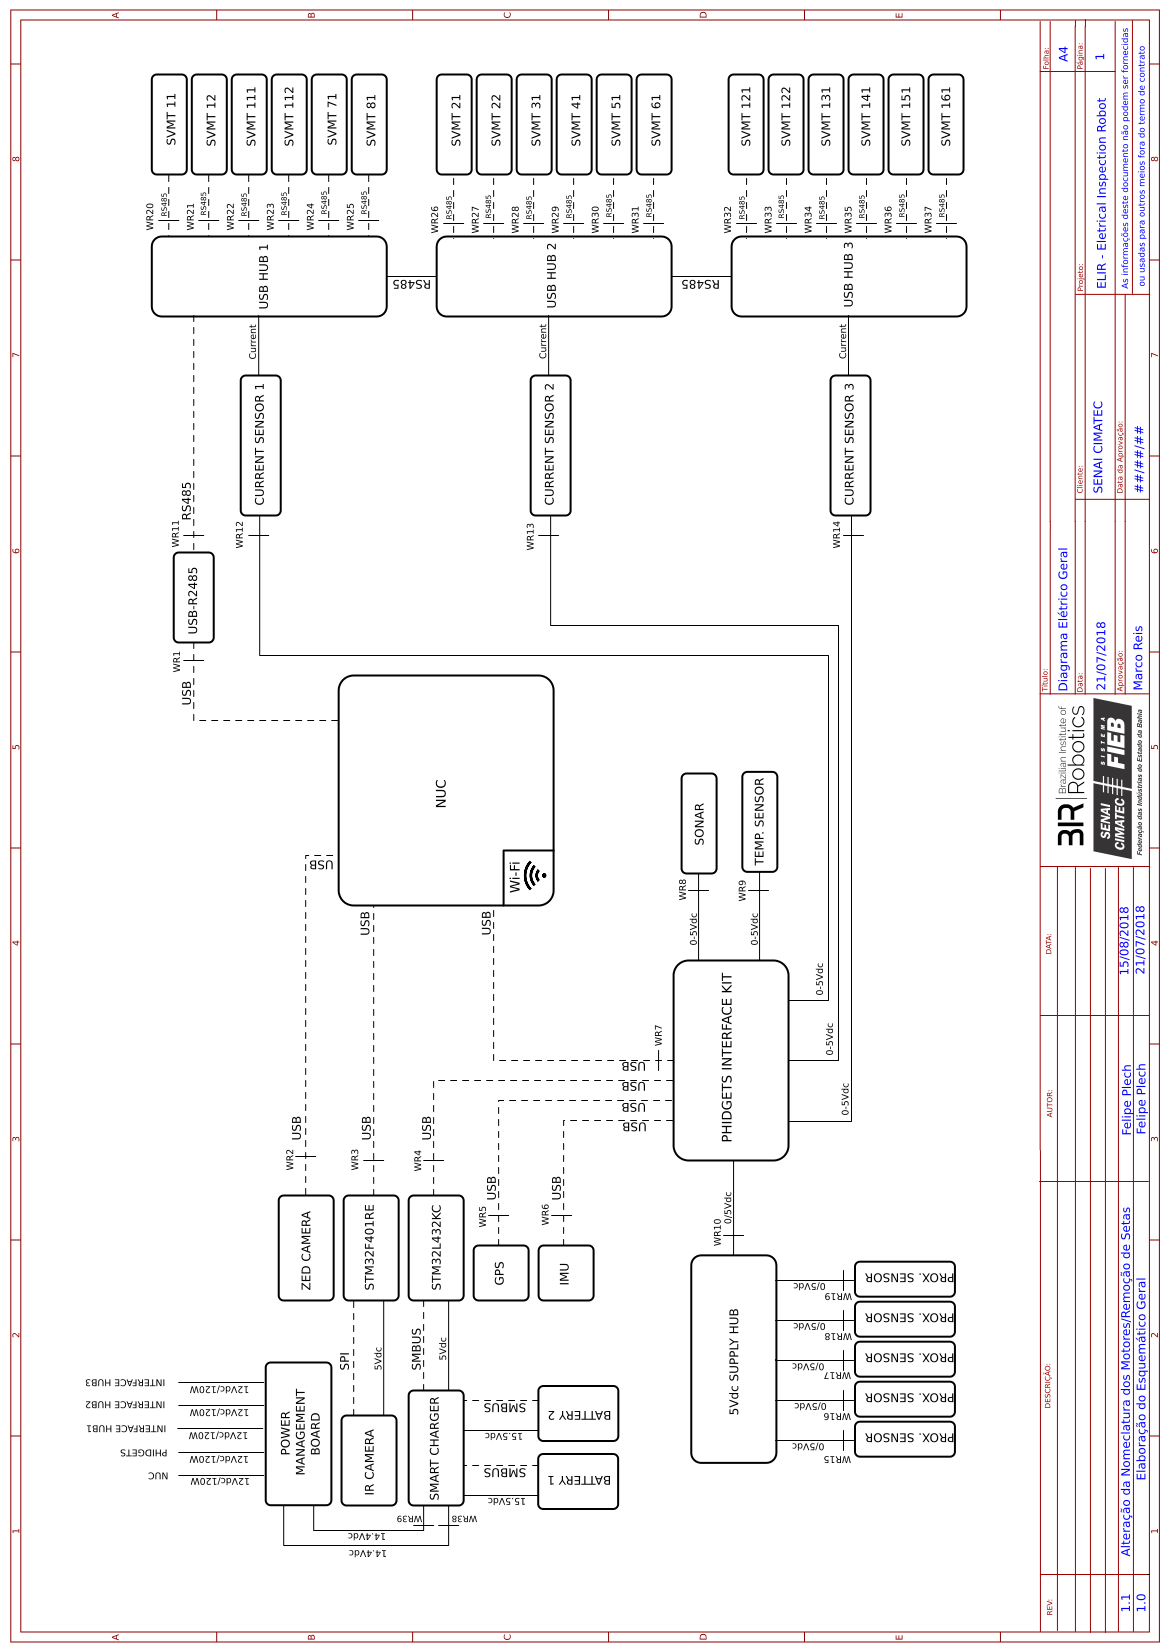
\includegraphics[width=14cm]{Figures/EsquematicoGeral.png}
	\caption{Esquemático Geral} \label{EGERAL}
	\end{figure}
	
    \pagebreak
    
    \begin{figure}[H]
	\centering
	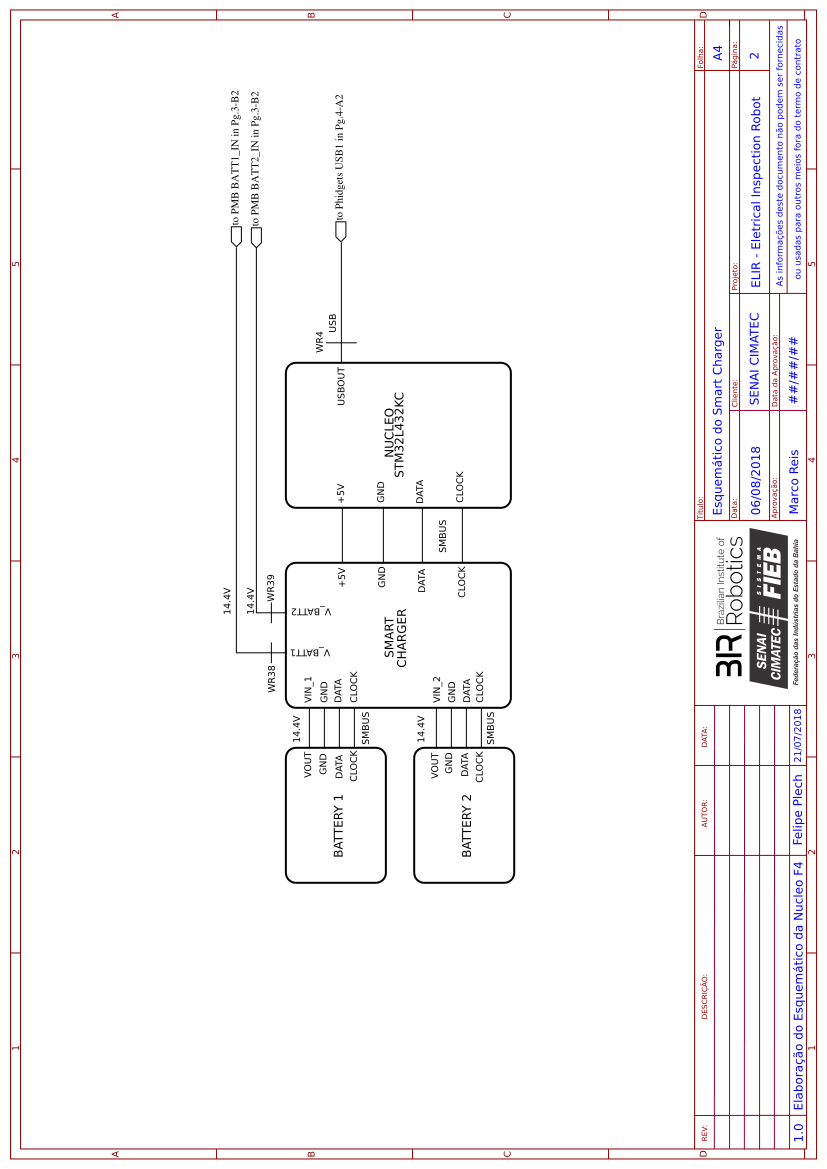
\includegraphics[width=14cm]{Figures/EsquematicoCHARGER.png}
	\caption{Esquemático - Smart Charger} \label{SmartCharger}
	\end{figure}
	
    \pagebreak
    
    \begin{figure}[H]
	\centering
	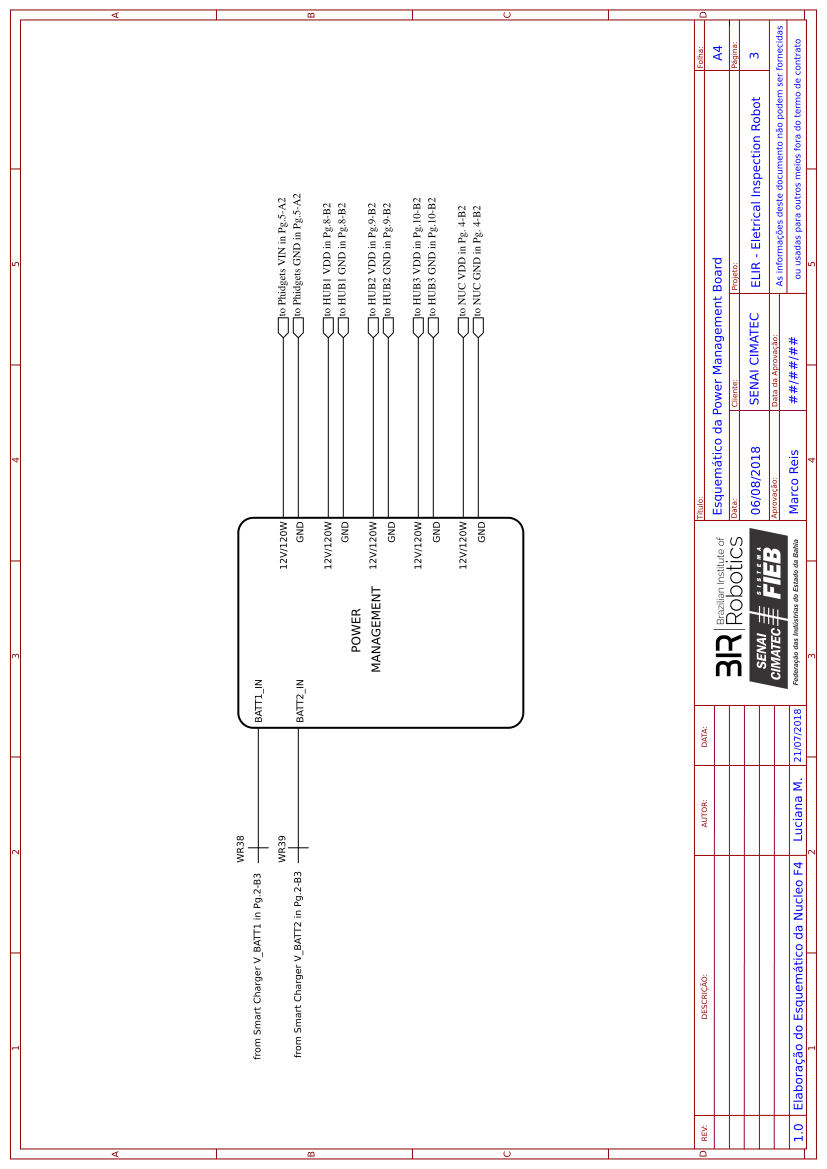
\includegraphics[width=14cm]{Figures/EsquematicoPMB.png}
	\caption{Esquemático - Placa de Gerenciamento de Energia} \label{PMB}
	\end{figure}
	
    \pagebreak
    
    \begin{figure}[H]
	\centering
	\includegraphics[width=14cm]{Figures/EsquematicoNUC.png}
	\caption{Esquemático - NUC} \label{NUC}
	\end{figure}
	
    \pagebreak
    
    \begin{figure}[H]
	\centering
	\includegraphics[width=14cm]{Figures/EsquematicoPHIDGETS.png}
	\caption{Esquemático - Phidgets} \label{Phidgets}
	\end{figure}
	
    \pagebreak
    
    \begin{figure}[H]
	\centering
	\includegraphics[width=14cm]{Figures/EsquematicoFLIR.png}
	\caption{Esquemático - STM32F401RE e FLIR LWIR Camera} \label{FLIR}
	\end{figure}
	
	\pagebreak
	
    \begin{figure}[H]
	\centering
	\includegraphics[width=14cm]{Figures/EsquematicoZED.png}
	\caption{Esquemático - ZED Camera} \label{ZED}
	\end{figure}
	
	\pagebreak
	
    \begin{figure}[H]
	\centering
	\includegraphics[width=14cm]{Figures/EsquematicoHUB1.png}
	\caption{Esquemático - HUB dos Atuadores 1} \label{HUB1}
	\end{figure}
	
	\pagebreak
	
    \begin{figure}[H]
	\centering
	\includegraphics[width=14cm]{Figures/EsquematicoHUB2.png}
	\caption{Esquemático - HUB dos Atuadores 2} \label{HUB2}
	\end{figure}
	
	\pagebreak
	
    \begin{figure}[H]
	\centering
	\includegraphics[width=14cm]{Figures/EsquematicoHUB3.png}
	\caption{Esquemático - HUB dos Atuadores 3} \label{HUB3}
	\end{figure}
	
	\pagebreak
	
    \begin{figure}[H]
	\centering
	\includegraphics[width=14cm]{Figures/board.png}
	\caption{Placa de Alimentação dos Sensores de Proximidade} \label{5vHUB}
	\end{figure}
        % Thesis Appendix -------------------------------------------------------

\chapter{Wireframes}
\label{Append:wireframes}

	\begin{figure}[!ht]
	\centering
	\includegraphics[width=14cm]{Figures/GUI_1.png}
	\caption{Dashboard - Main page} \label{UI}
	\end{figure}
	
	\begin{figure}[!ht]
	\centering
	\includegraphics[width=16cm]{Figures/GUI_2.jpg}
	\caption{Dashboard - Actuators Info Page} \label{UI2}
	\end{figure}


        % Thesis Appendix -------------------------------------------------------

\chapter{Logbook}
\label{Append:log}



    \end{thesisappendices}

    %%----------------------------------------------------------------------------
    %% Configurar as referencias bibliograficas
    %%----------------------------------------------------------------------------


    \addcontentsline{toc}{chapter}{Referências}
    %\bibliographystyle{abnt-alf}


    \bibliography{References/referencias}

    %%----------------------------------------------------------------------------
    %% Finishing
    %%----------------------------------------------------------------------------

    \include{Others/ultimafolha}
\end{document}
%%%-------------------------------------------------------------------------------
%%% Here we finished with your thesis formating. Good luck with the contents
%%%-------------------------------------------------------------------------------
